
\chapter{Kronecker's Limit Formulas}\label{chap1}

\section{The first limit formula}\label{chap1:sec1}\pageoriginale

Let $s=\sigma + it$ be a complex variable, $\sigma$ and $t$ being
real. The Riemann zeta-function $\zeta(s)$ is defined for $\sigma>1$
by
$$
\zeta(s)=\sum^{\infty}_{k=1}k^{-s},
$$
here $k^{-s}$ stands for $e^{-s\log k}$, with the real value of $\log
k$. The series converges absolutely for $\sigma>1$ and uniformly in
every $s$-half-plane defined by $\sigma\geq
1+\varepsilon(\varepsilon>0)$. It follows from a theorem of Weierstrass that
the sum-function $\zeta(s)$ is a regular function of $s$ for
$\sigma>1$. Riemann proved that $\zeta(s)$ possesses an analytic
continuation into the whole $s$-plane which is regular except for a
simple pole at $s=1$ and satisfies the well-known functional equation
$$
\pi^{-s/2}\Gamma\left(\frac{s}{2}\right)\zeta(s)=\pi^{-((1-s)/2)}\Gamma\left(\frac{1-s}{2}\right)\zeta(1-s), 
$$
$\Gamma(s)$ being Euler's gamma-function.

We shall now prove

\begin{proposition}\label{prop1}
The function $\zeta(s)$ can be continued analytically into the
half-plane $\sigma>0$ and the continuation is regular for $\sigma>0$,
except for a simple pole at $s=1$ with residue $1$. Further, at $s=1$,
$\zeta(s)$ has the expansion
$$
\zeta(s)-\frac{1}{s-1}=C+a_{1}(s-1)+a_{2}(s-1)^{2}+\cdots
$$
$C$ being Euler's constant.
\end{proposition}

We first need to prove the simplest form of a summation formula due to
Euler, namely.

\begin{lemma*}
If $f(x)$ is a complex-valued function having a continuous deri\-vative
$f'(x)$ in the interval $1\leq x\leq n$, then 
\begin{gather*}
\int^{1}_{0}\left(\sum^{n-1}_{k=1}f'(x+k)\left(x-\frac{1}{2}\right)\right)dx+\frac{f(1)+f(n)}{2}\\ 
=\sum^{n}_{k=1}f(k)-\int^{n}_{1}f(x)dx.\tag{1}\label{1}
\end{gather*}\pageoriginale
\end{lemma*}

\begin{proof}
In fact, if a complex-valued function $g(x)$ defined in the interval
$0\leq x\leq 1$, has a continuous derivative $g'(x)$, then we have
from integration by parts,
\begin{equation*}
\int^{1}_{0}g'(x)\left(x -
\frac{1}{2}\right)dx=\frac{1}{2}(g(0)+g(1))-\int^{1}_{0}g(x)dx.\tag{2}\label{2}  
\end{equation*}
(Formula \eqref{2} has a simple geometric interpretation in that the
right hand side of \eqref{2} represents the area of the portion of the
$(x,y)$-plane bounded by the curve $y=g(x)$ and the straight lines
$y-g(0)=(g(1)-g(0))x$, $x=g(0)$ and $x=g(1)$). In \eqref{2}, we now
set $g(x)=f(x+k)$, successively for $k=1,2,\ldots,n-1$. We then have
for $k=1,2,\ldots,n-1$, 
$$
\int^{1}_{0}f'(x+k)\left(x-\frac{1}{2}\right)dx=\frac{1}{2}(f(k)+f(k+1))-\int^{k+1}_{k}f(x)dx. 
$$
Adding up, we obtain formula (1).
\end{proof}

This is Euler's summation formula in its simplest form, with the
remainder term involving only the first derivative of $f(x)$.

It is interesting to notice that if one uses the fact that the Fourier
series $-\sum\limits_{n}\dfrac{e^{2\pi inx}}{2\pi in}$ ($n=0$,
omitted) converges uniformly to $x-1/2$ in any closed interval
$(\epsilon,1-\epsilon)(0<\epsilon<1)$ one obtains from \eqref{2} the
following useful result, namely,

{\em If $f(x)$ is periodic in $x$ with period $1$ and has a continuous
  derivative, then}
$$
f(x)=\sum^{\infty}_{n=-\infty}e^{2\pi in x}\int^{1}_{0}f(x)e^{-2\pi in
  x}dx.
$$

\begin{proofofprop}\label{proofofprop1}
Let us now specialize $f(x)$ to be the function $f(x)=x^{-s} = e^{-s\log
  x}$ ($\log x$ taking real values for $x>0$). The
function\pageoriginale $x^{-s}$ is evidently continuously
differentiable in the interval $1\leq x\leq n$; and applying \eqref{1}
to the function $x^{-s}$, we get
\begin{align*}
&-
  s\sum^{n-1}_{k=1}\int^{1}_{0}(x+k)^{-s-1}\left(x-\frac{1}{2}\right)dx+\frac{1}{2}(1+n^{-s})\\
&=\sum^{n}_{k=1}k^{-s}-\int^{n}_{1}x^{-s}dx\\
&=
\begin{cases}
\sum^{n}_{k=1}k^{-s}-\frac{1-n^{1-s}}{s-1}(\text{if } s\neq 1)\\
\sum^{n}_{k=1}k^{-1}-\log n(\text{if }s=1).
\end{cases}\tag{3}\label{3}
\end{align*}
Let us now observe that the right-hand side of \eqref{3} is an entire
function of $s$.
\end{proofofprop}

We suppose now that $\sigma>1$. When $n$ tends to infinity
$\int^{n}_{1}x^{-s}dx$ tends to $1/(s-1)$. Further, as $n$ tends to
infinity, $\sum\limits^{n}_{k=1}k^{-s}$ converges to $\zeta(s)$. Thus
for $\sigma>1$, the right hand side of \eqref{3} converges to
$\zeta(s)-1/(s-1)$ as $n$ tends to infinity.

On the other hand, let the left-hand side of \eqref{3} be denoted by
$\varphi_{n}(s)$. Then $\varphi_{n}(s)$ is an entire function of $s$
and further, for $\sigma\geq\epsilon>0$,
\begin{align*}
|\varphi_{n}(s)| &\leq
\frac{1}{2}|s|\sum^{n}_{k=1}k^{-1-\epsilon}+\frac{1+n^{-\epsilon}}{2}\\
&\leq \frac{1}{2}|s|\sum^{\infty}_{k=1}k^{-1-\epsilon}+1.
\end{align*}
Thus, as $n$ tends to infinity, $\varphi_{n}(s)$ converges to a
regular function of $s$ in the half-plane $\sigma>0$; this provides
the analytic continuation of $\zeta(s)-1/(s-1)$ for $\sigma>0$.

Now the constant $a_{0}$ in the power-series expansion at $s=1$ of 
$$
\zeta(s)-\frac{1}{s-1}=a_{0}+a_{1}(s-1)+a_{2}(s-1)^{2}+\cdots
$$
is nothing but $\lim\limits_{n\to \infty}\varphi_{n}(1)$. In other
words, 
\begin{align*}
a_{\circ}  & = 
\lim\limits_{n\to\infty}\left(1+\frac{1}{2}+\cdots+\frac{1}{n}-\log
n\right)\\
&= C\text{ (Euler's constant).}
\end{align*}\pageoriginale
Proposition \ref{prop1} is thus proved.

The constant $C$ lies between $0$ and $1$. It is not known whether it
is rational or irrational; very probably, it is irrational.

One could determine the constants $a_{1},a_{2},\ldots$ also explicitly
but this is more complicated.

We shall consider now an analogous problem leading to the {\bf
  Kronecker limit formula} (Kroneckersche Grenzformel).

Instead of the simple linear function $x$, we consider a
positive - definite binary quadratic form $Q(u,v)=au^{2}+2buv+cv^{2}$ in
the {\em real} variables $u$ and $v$ and with {\em real} coefficients
$a$, $b$, $c$ (we then have $a>0$ and $ac-b^{2}=d>0$). Associated with
$Q(u,v)$, let us define
\begin{equation*}
\zeta_{Q}(s)=\sum^{\infty}_{m,n=-\infty}(Q(m,n))^{-s},\tag{4}\label{4}
\end{equation*}
where $\sum'$ denotes summation over all pairs of integers $(m,n)$,
except $(0,0)$.

$Q(u,v)$ being positive-definite, there exists a real number
$\lambda>0$, such that $Q(u,v)\geq \lambda (u^{2}+v^{2})$ and it is an
immediate consequence that the series \eqref{4} converges absolutely
for $\sigma>1$ and uniformly in every half-plane defined by
$\sigma\geq 1+\epsilon(\epsilon>0)$. Thus $\zeta_{Q}(s)$ is a regular
function of $s$, for $\sigma>1$.

As in the case of $\zeta(s)$ above, we shall obtain an analytic
continuation of $\zeta_{Q}(s)$ regular in the half-plane $\sigma>1/2$,
except for a simple pole at $s=1$. The constant $a_{0}$ in the
expansion at $s=1$ of $\zeta_{Q}(s)$, viz.
$$
\zeta_{Q}(s)=\frac{a_{-1}}{s-1}+a_{0}+a_{1}(s-1)+\cdots
$$
is given precisely by the Kronecker limit formula. The constant
$a_{-1}$ which is the residue of $\zeta_{Q}(s)$ at $s=1$ was found by
Dirichlet in his investigations on the class-number of quadratic
fields.

Let\pageoriginale us first effect some simplifications.

Since $Q(u,v)=Q(-u,-v)$, we see that
\begin{equation*}
\zeta_{Q}(s)=2\sum^{\infty}_{m=1}(Q(m,0))^{-s}+2\sum^{\infty}_{n=1}\sum^{\infty}_{m=-\infty}(Q(m,n))^{-s}.\tag{5}\label{5} 
\end{equation*}
Further
\begin{align*}
Q(u,v) &=
a\left(u+\frac{b}{a}v\right)^{2}+\left(c-\frac{b^{2}}{a}\right)v^{2}\\
&=
a\left(u+\frac{b}{a}v\right)^{2}+\frac{d}{a}v^{2}=a\left(u+\frac{b+\sqrt{-d}}{a}v\right)\left(u+\frac{b-\sqrt{-d}}{a}v\right)\\
&= a(u+zv)(u+\ob{z}v)
\end{align*}
where $\arg(\sqrt{-d})=\pi/2$ and $z=(b+\sqrt{-d})/a=x+iy$ with
$y>0$. 

Also, we could, without loss of generality, suppose that $d=1$; if
$Q_{1}(u,v)=(1/\sqrt{d})(au^{2}+2buv+cv^{2})=a_{1}u^{2}+2b_{1}uv+c_{1}v^{2}$,
then $\zeta_{Q_{1}}(s)=d^{s/2}\zeta_{Q}(s)$ and
$a_{1}c_{1}-b^{2}_{1}=1$. The function $d^{s/2}$ (choosing a fixed
branch) is a simple entire function of $s$ and therefore, to study
$\zeta_{Q}(s)$, it is enough to consider $\zeta_{Q_{1}}(s)$. Then we
have $a=y^{-1}$ and
$Q(u,v)=y^{-1}(u+zv)(u+\ob{z}v)=y^{-1}|u+zv|^{2}$. Now \eqref{5}
becomes
\begin{align*}
\zeta_{Q}(s) &=
2y^{s}\sum^{\infty}_{m=1}m^{-2s}+2y^{s}\sum^{\infty}_{n=1}\sum^{\infty}_{m=-\infty}|m+nz|^{-2s}\\
&=
2y^{s}\zeta(2s)+2y^{s}\sum^{\infty}_{n=1}\sum^{\infty}_{m=-\infty}|m+nz|^{-2s}\tag{6}\label{6} 
\end{align*}

We know from Proposition \ref{prop1} that $\zeta(2s)$ has an analytic
continuation in the half-plane $\sigma>0$, regular except for a simple
pole at $s=1/2$. To obtain an analytic continuation for
$\zeta_{Q}(s)$, we have, therefore, only to investigate the nature of
the second term on the right hand side of \eqref{6}, as a function of
$s$. For this purpose, we need the {\bf Poisson summation formula.}

\begin{proposition}\label{prop2}
Let $f(x)$ be continuous in $(-\infty,\infty)$ and let
$\sum\limits^{\infty}_{m=-\infty}f(x+m)$ be uniformly convergent in
$0\leq x\leq 1$. Then 
$$
\sum^{\infty}_{m=-\infty}f(x+m)=\sum^{\infty}_{k=-\infty}e^{-2\pi
  ikx}\int\limits^{\infty}_{-\infty}f(\xi)e^{2\pi ik\xi}d\xi.
$$\pageoriginale
\end{proposition}

\begin{proof}
The function $\varphi(x)=\sum\limits^{\infty}_{m=-\infty}f(x+m)$ is
continuous in $(-\infty,\infty)$ and periodic in $x$, of period
$1$. If $a_{k}=\int^{1}_{0}\varphi(\xi)e^{2\pi ik\xi}d\xi$ then, by
F\'ej\'er's Theorem, the $(C,1)$ sum of
$\sum\limits^{\infty}_{k=-\infty}a_{k}e^{-2\pi ikx}$ is equal to
$\varphi(x)$. In particular, if
$\sum\limits^{\infty}_{k=-\infty}|a_{k}|$ converges, then for $x$ in
$(-\infty,\infty)$ 
$$
\sum^{\infty}_{m=-\infty}f(x+m)=\varphi(x)=\sum^{\infty}_{k=-\infty}e^{-2\pi
  ikx}\int^{1}_{0}\varphi(\xi)e^{2\pi ik\xi}d\xi. 
$$
In view of the uniform convergence of
$\sum\limits^{\infty}_{m=-\infty}f(x+m)$ in $0\leq x\leq 1$,
\begin{align*}
\int^{1}_{0}\sum^{\infty}_{m=-\infty}f(\xi+m)e^{2\pi ik\xi}d\xi &=
\sum^{\infty}_{m=-\infty}\int^{1}_{0}f(\xi+m)e^{2\pi ik\xi}d\xi\\
&= \int^{\infty}_{-\infty}f(\xi)e^{2\pi ik\xi}d\xi.
\end{align*}
Thus
\begin{equation*}
\sum^{\infty}_{m=-\infty}f(x+m)=\sum^{\infty}_{k=-\infty}e^{-2\pi
  ikx}\int^{\infty}_{-\infty}f(\xi)e^{2\pi ik\xi}d\xi,\tag{7}\label{7}
\end{equation*}
which is the Poisson summation formula.

Now we set $f(x)=|x+iy|^{-2s}=|z|^{-2s}$ for $x$ in
$(-\infty,\infty)$. Then we see that the series
$\sum\limits^{\infty}_{m=-\infty}|m+z|^{-2s}$ converges absolutely,
uniformly in every interval $-N\leq x\leq N$, for $\sigma>1/2$. For
this purpose, it clearly suffices to consider the interval $0\leq
x\leq 1$, since the series remains unchanged when $x$ is replaces by
$x+1$. For $0\leq x\leq 1$,
\begin{align*}
&\left| \sum^{\infty}_{m=-\infty}|m+z|^{-2s}\right|\leq
  \sum^{\infty}_{m=-\infty}|m+z|^{-2\sigma}\\
&\leq
  |z|^{-2\sigma}+|z-1|^{-2\sigma}+\sum^{\infty}_{m=1}(m^{-2\sigma}+m^{-2\sigma})
  \\
&<2y^{-2\sigma}+2\sum^{\infty}_{m=1}m^{-2\sigma}\left(\sigma>\frac{1}{2}\right).
\end{align*}\pageoriginale
\end{proof}

Thus, by \eqref{7}, for $\sigma>1/2$,
\begin{align*}
\sum^{\infty}_{m=-\infty}|m+z|^{-2s} &=
\sum^{\infty}_{k=-\infty}e^{-2\pi
  ikx}\int^{\infty}_{-\infty}|\xi+iy|^{-2s}e^{2\pi ik\xi}d\xi\\
&= \sum^{\infty}_{k=-\infty}e^{-2\pi
  ikx}\int^{\infty}_{-\infty}(\xi^{2}+y^{2})^{-s}e^{2\pi ik\xi}d\xi\\
&= y^{1-2s}\sum^{\infty}_{k=-\infty}e^{-2\pi
  ikx}\int^{\infty}_{-\infty}(1+\xi^{2})^{-s}e^{2\pi ik\xi}d\xi,\tag{8}\label{8}
\end{align*}
whenever the series \eqref{8} converges. Actually, we shall prove that
it converges absolutely for $\sigma>1/2$. For this purpose, let us
consider for $k>0$, $\int^{\infty}_{-\infty}(1+\zeta^{2})^{-s}e^{2\pi
  ik\zeta}d\zeta$ as a line integral in the complex $\zeta$-plane; let
$\zeta=\xi+i\eta$. The function $(1+\zeta^{2})^{-s}$ has a logarithmic
branch-point at $\zeta=i$ and $\zeta=-i$. In the complex $\zeta$-plane
cut along the $\eta$-axis from $\eta=1$ to $\eta=\infty$ and from
$\eta=-1$ to $\eta=-\infty$, let $ABCDEFG$ denote the contour
consisting of the straight line $GA(\eta=0,|\xi|\leq R)$, the arc
$AB(\zeta=R e^{i\theta} \; \pi\geq \theta\geq \pi/2)$, the straight line
$BC(\xi=0, 3/2\leq \eta\leq R)$ on the left bank of the cut, the
circle
$$
CDE(\zeta=i+(i/2)e^{i\varphi}, 0\leq \varphi\leq 2\pi),
$$
the straight line $EF$ on the right bank of the cut $(\xi=0,3/2\leq
\eta\leq R)$ 
\begin{figure}[H]
\centering
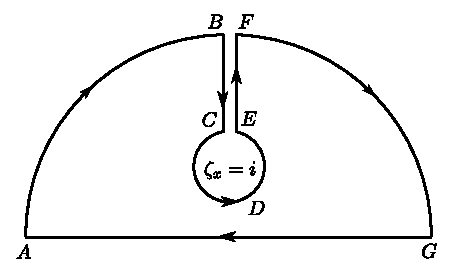
\includegraphics{fig1.eps}

\medskip
\centerline{\bf Fig.~1}
\end{figure}
and\pageoriginale the arc $FG(\zeta=R e^{i\theta},\pi/2\geq \theta\geq
0)$. If $s$ lies in a compact set $K$ of the $s$-plane with
$\sigma>0$, then on the arcs $AB$ and $FG$,
\begin{align*}
|(1+\zeta^{2})^{-s}e^{2\pi iky\zeta}| &\leq
|1+\zeta^{2}|^{-\sigma}e^{-2\pi ky}R\sin \theta\\
&= O(R^{-2\sigma}e^{-2\pi ky \ R\sin \theta}),
\end{align*}
since $-\pi \leq \arg(1+\zeta^{2})\leq \pi$ on the whole contour. The
constants in the $O$-estimate depend only on $K$. Thus
\begin{align*}
\left| \int_{AB}(1+\zeta^{2})^{-s}e^{2\pi iky\zeta}d\zeta\right| &=
O \left(R^{-2\sigma}\int^{\pi/2}_{0}e^{-2\pi ky\ R\sin
  \theta}Rd\theta\right)\\
&= O \left(R^{1-2\sigma}\int^{\pi/2}_{0}e^{-4ky
  R\theta}d\theta\right)\\
&= O (R^{-2\sigma}),
\end{align*}
and hence $\int_{AB}(1+\zeta^{2})^{-s}e^{2\pi ik\zeta}d\zeta$ tends to
zero as $R$ tends to infinity. Similarly
$\int_{FG}(1+\zeta^{2})^{-s}e^{2\pi ik\zeta}d\zeta$ also tends to zero
as $R$ tends to infinity. If $\Gamma^{+}$ denotes the contour $BCDEF$
in the limiting position as $R$ tends to infinity, then for
$\sigma>0$, we have, by Cauchy's Theorem,
\begin{equation*}
\int^{\infty}_{-\infty}(1+\zeta^{2})^{-s}e^{2\pi
  iky\zeta}d\zeta=\int_{\Gamma^{+}}(1+\zeta^{2})^{-s}e^{2\pi
  iky\zeta}d\zeta.\tag{9} \label{9}
\end{equation*}

Let $\Gamma^{-}$ denote the limiting position of $B'C'D'E'F'$ (which
is the reflection of $BCDEF$ with respect to $\xi$-axis), as $R$ tends
to infinity. We can show similarly that when $k<0$,
\begin{equation*}
\int^{\infty}_{-\infty}(1+\zeta^{2})^{-s}e^{2\pi
  iky\zeta}d\zeta=\int_{\Gamma^{-}}(1+\zeta^{2})^{-s}e^{2\pi
  iky\zeta}d\zeta.\tag{10}\label{10} 
\end{equation*}

We shall now show that the right hand side of \eqref{9} defines an
entire function of $s$. In fact, if $s=\sigma+it$ lies in a compact
set $K$ in the $s$-plane with $\sigma>-d(d>0)$, then, on $\Gamma^{+}$
we have for a constant $c_{1}$ depending only on $K$,
$|1+\zeta^{2}|^{-\sigma}\leq c_{1}\eta^{2d}$. Thus for $k>0$,
\begin{align*}
& \left|\int_{\Gamma^{+}}(1+\zeta^{2})^{-s}e^{2\pi
  iky\zeta}d\zeta\right|\leq
\int\limits_{\Gamma^{+}}|(1+\zeta^{2})^{-s}|e^{-2\pi ky\eta}|d\zeta|\\
&\leq \int_{\Gamma^{+}}|1+\zeta^{2}|^{-\sigma}e^{\pi|t|-2\pi
  ky\eta}|d\zeta|\leq c_{1}\int_{\Gamma^{+}}\eta^{2d}e^{\pi |t|-2\pi
  ky\eta}|d\zeta|\\
&\leq c_{2}e^{-\pi ky}\int_{\Gamma^{+}}\eta^{2d}e^{-2\pi
  ky(\eta-\frac{1}{2})}|d\zeta|\leq c_{2}e^{-\pi
  ky}\int_{\Gamma^{+}}\eta^{2d}e^{-2\pi y(\eta-\frac{1}{2})}|d\zeta|\\
&\leq c_{3}e^{-\pi ky},\tag{11}\label{11}
\end{align*}\pageoriginale
the constants $c_{2}$ and $c_{3}$ depending only on $K$. Hence
$\int_{\Gamma^{+}}(1+\zeta^{2})^{-s}\break e^{2\pi ky\zeta}d\zeta$ converges
absolutely and uniformly in $K$ and therefore defines an analytic
function of $s$ in any domain contained in $K$. Since $d$ is an
arbitrary positive number, our assertion above is proved. Similar to
\eqref{11}, we have also for $k<0$,
\begin{equation*}
\left|\int_{\Gamma^{-}}(1+\zeta^{2})^{-s}e^{2\pi
  iky\zeta}d\zeta\right|\leq c'_{3}e^{-\pi|k|y},\tag{12}\label{12}
\end{equation*}
and therefore $\int_{\Gamma^{-}}(1+\zeta^{2})^{-s}e^{2\pi
  iky\zeta}d\zeta$ defines for $k<0$, an entire function of $s$.

In view of \eqref{9}, \eqref{10}, \eqref{11} and \eqref{12}, we see
that in order to prove the absolute convergence of the series
\eqref{8}, for $\sigma>1/2$, we need to prove only that for
$\sigma>1/2$, $\int^{\infty}_{-\infty}(1+\zeta^{2})^{-s}d\zeta$
exists. But, in fact, for $\sigma>1/2$,
\begin{align*}
\int^{\infty}_{-\infty}(1+\zeta^{2})^{-s}d\zeta &=
2\int^{\infty}_{0}(1+\zeta^{2})^{-s}d\zeta\\ 
&=
\int^{\infty}_{0}(1+\lambda)^{-s}\lambda^{-\frac{1}{2}}d\lambda\quad
(\text{setting } \zeta^{2}=\lambda)\\
&=
\int^{1}_{0}\mu^{-\frac{1}{2}}(1-\mu)^{s-3/2}d\mu\left(\text{setting
}\lambda=\frac{\mu}{1-\mu}\right)\\
&= B\left(\frac{1}{2},s-\frac{1}{2}\right), 
\end{align*}
where $B(a,b)$ is Euler's beta-function. Hence
$$
\int^{\infty}_{-\infty}(1+\zeta^{2})^{-s}d\zeta=\frac{\pi^{\frac{1}{2}}\Gamma(s-\frac{1}{2})}{\Gamma(s)} 
$$
Thus, for $\sigma>1$, 
{\fontsize{10}{12}\selectfont
$$
\sum^{\infty}_{m=-\infty}|m+z|^{-2s}=\frac{\pi^{\frac{1}{2}}\Gamma(s-\frac{1}{2})}{\Gamma(s)}y^{1-2s}+y^{1-2s}\mathop{{\sum}'}^{\infty}_{m=-\infty}
e^{-2\pi imx}\int^{\infty}_{-\infty}(1+\zeta^{2})^{-s}e^{2\pi
  imy\zeta}d\zeta, 
$$}\pageoriginale
where the accent on $\Sigma$ indicates the omission of
$m=0$. Substituting this in \eqref{6}, we have for $\sigma>1$,
\begin{align*}
\zeta_{Q}(s) &= 2y^{s}\zeta(2s)+\\
  &\quad
  +2y^{s}\sum^{\infty}_{n=1}\left\{\frac{\pi^{\frac{1}{2}}\Gamma(s-\frac{1}{2})}{\Gamma(s)}n^{1-2s}y^{1-2s}+n^{1-2s}y^{1-2s}\times\right.\\
&\qquad\quad \left.\times
  \mathop{{\sum}'}^{\infty}_{m=-\infty}e^{-2\pi
    imnx}\int^{\infty}_{-\infty}(1+\zeta^{2})^{-s}e^{2\pi imny\zeta}d\zeta\right\}
\end{align*}
By \eqref{9} and \eqref{10}, therefore, for $\sigma>1$,
\begin{align*}
\zeta_{Q}(s) &=
2y^{s}\zeta(2s)+2y^{1-s}\frac{\pi^{\frac{1}{2}}\Gamma(s-\frac{1}{2})}{\Gamma(s)}\zeta(2s-1)+\\
&\quad
+2y^{1-s}\sum^{\infty}_{n=1}n^{1-2s}\sum^{\infty}_{m=-\infty}e^{-2\pi
  imnx}\int^{\infty}_{-\infty}(1+\zeta^{2})^{-s}e^{2\pi
  imny\zeta}d\zeta; 
\end{align*}
\ie
\begin{align*}
\zeta_{Q}(s) &=
2y^{s}\zeta(2s)+2y^{1-s}\frac{\pi^{\frac{1}{2}}\Gamma(s-\frac{1}{2})}{\Gamma(s)}\zeta(2s-1)+2y^{1-s}\sum^{\infty}_{n=1}n^{1-2s}\times\\
&\quad \times \left\{\sum^{\infty}_{m=1}e^{-2\pi
  imnx}\int_{\Gamma^{+}}(1+\zeta^{2})^{-s}e^{2\pi
  imny\zeta}d\zeta+\right.\\
&\qquad \left.\sum^{\infty}_{m=1}e^{2\pi
  imnx}\int_{\Gamma^{-}}(1+\zeta^{2})^{-s}e^{-2\pi
  imny\zeta}d\zeta\right\}.\tag{13}\label{13} 
\end{align*}
The double series in \eqref{13} converges absolutely, uniformly in
every compact subset of the $s$-plane, in view of the fact that by
\eqref{11} and \eqref{12}, it is majorised by
$$
2y^{1-\sigma}\sum^{\infty}_{n=1}n^{1-2\sigma}\left(c_{3}\sum^{\infty}_{m=1}e^{-\pi
  mny}+c'_{3}\sum^{\infty}_{m=1}e^{-\pi mny}\right), 
$$
which\pageoriginale clearly converges. Since we have seen earlier that
the terms of the double series define entire functions of $s$, it
follows by the theorem of Weierstrass that the double series in
\eqref{13} defines an entire function of $s$.

Formula \eqref{13} gives us an analytic continuation of $\zeta_{Q}(s)$
for $\sigma>1/2$. For, $\zeta(2s)$ is regular for $\sigma>1/2$ and
from the fact that $\zeta(s)$ can be analytically continued into the
half-plane $\sigma>0$ such that $\zeta(s)-1/(s-1)$ is regular for
$\sigma>0$, we see on replacing $s$ by $2s-1$ that $\zeta(2s-1)$ can
be continued analytically in the half-plane $\sigma>1/2$ such that
$\zeta(2s-1)-1/2(s-1)$ regular for
$\sigma>1/2:\Gamma(s-\frac{1}{2})/\Gamma(s)$ is regular for
$\sigma>1/2$ and non-zero at $s=1$. Hence from \eqref{13}, we see that
$\zeta_{Q}(s)$ can be continued analytically in the half-plane
$\sigma>1/2$ and its only singularity in this half-plane is a simple
pole at $s=1$ with residue equal to $2\cdot \pi^{\frac{1}{2}}\cdot
\pi^{\frac{1}{2}}\cdot 1/2=\pi$. 

$\zeta_{Q}(s)-\pi/(s-1)$ has therefore a convergent power-series
expansion $a_{0}+a_{1}(s-1)+\cdots$ at $s=1$. We shall now determine
the constant $a_{0}$. Clearly, from \eqref{13},
\begin{align*}
a_{0}&= 2y\zeta(2)+\lim\limits_{s\to
  1}\left(2y^{1-s}\frac{\pi^{\frac{1}{2}}\Gamma(s-\frac{1}{2})}{\Gamma(s)}\zeta(2s-1)-\frac{\pi}{s-1}\right)
+\\
&\quad
+2\sum^{\infty}_{n=1}\frac{1}{n}\left(\sum^{\infty}_{m=1}e^{-2\pi
  imnx}\int_{\Gamma^{+}}(1+\zeta^{2})^{-1}e^{2\pi
  imny\zeta}d\zeta+\right.\\
&\qquad \left. +\sum^{\infty}_{m=1}e^{2\pi
  imnx}\int_{\Gamma^{-}}(1+\zeta^{2})^{-1}e^{-2\pi imny\zeta}d\zeta\right)
\end{align*}
Now from
$$
\zeta(s)=\frac{1}{s-1}+C+a_{1}(s-1)+\cdots
$$
we have
$$
\zeta(2s-1)=\frac{1}{2(s-1)}+C+2a_{1}(s-1)+\cdots.
$$
Also replacing $s$ by $s-1/2$ in the formula
$$
\Gamma\left(s+\frac{1}{2}\right)\Gamma(s)=\sqrt{\pi}\cdot
2^{1-2s}\Gamma(2s).
$$
we\pageoriginale have
$$
\Gamma\left(s-\frac{1}{2}\right)\Gamma(s)=\sqrt{\pi}2^{2-2s}\Gamma(2s-1).
$$
At $s=1$, $\Gamma(s)$ has the expansion
$$
\Gamma(s)=1+a(s-1)+\cdots
$$
and hence
$$
\Gamma^{2}(s)=1+2a(s-1)+\cdots
$$
Further at $s=1$,
$$
\Gamma(2s-1)=1+2a(s-1)+\cdots
$$
Hence we have at $s=1$, by Cauchy multiplication of power-series,
$$
\Gamma(2s-1)\Gamma^{-2}(s)=1+b(s-1)^{2}+\cdots
$$
and thus
\begin{align*}
2y^{1-s}\pi^{\frac{1}{2}}\frac{\Gamma(s-\frac{1}{2})}{\Gamma(s)}\zeta(2s-1)
&= 2\pi
(2\sqrt{y})^{2-2s}\frac{\Gamma(2s-1)}{\Gamma^{2}(s)}\zeta(2s-1)\\
&= 2\pi(1+b(s-1)^{2}+\cdots)\times\\
&\quad \times(1-2\log(2\sqrt{y})(s-1)+\cdots)\times\\
&\quad \times\left(\frac{1}{2(s-1)}+C+\cdots\right).
\end{align*}
In other words,
$$
\lim\limits_{s\to
  1}\left(2y^{1-s}\pi^{\frac{1}{2}}\frac{\Gamma(S-\frac{1}{2})}{\Gamma(s)}\zeta(2s-1)-\frac{\pi}{s-1}\right)=2\pi(C-\log(2\sqrt{y})) 
$$
Now (see Fig.\@ 1), for $mn>0$, since $(1+\zeta^{2})^{-1}$ has no
branch-point at $\zeta=i$ or $\zeta=-i$,
\begin{align*}
\int_{\Gamma^{+}}(1+\zeta^{2})^{-1}e^{2\pi imny\zeta}d\zeta &=
\int_{CDE}(1+\zeta^{2})^{-1}e^{2\pi imny\zeta}d\zeta\\
&= 2\pi i\left(\text{Residue of } \frac{e^{2\pi
    imny\zeta}}{1+\zeta^{2}}\text{ at } \zeta=i\right)\\
&= \pi e^{-2\pi mny}.
\end{align*}\pageoriginale
Similarly, for $mn>0$,
\begin{align*}
\int_{\Gamma^{-}}(1+\zeta^{2})^{-1}e^{-2\pi imny\zeta}d\zeta &= -2\pi
i\left(\text{Residue of } \frac{e^{-2\pi
    imny\zeta}}{1+\zeta^{2}}\text{ at } \zeta=-i\right)\\
&= \pi e^{-2\pi mny}
\end{align*}
Hence
\begin{align*}
a_{0}=\frac{\pi^{2}}{3}y+2\pi(C-\log(2\sqrt{y})) &+ 2\pi
\sum^{\infty}_{n=1}\frac{1}{n}\sum^{\infty}_{m=1}e^{-2\pi imnx-2\pi
  mny}+\\
&+ 2\pi \sum^{\infty}_{n=1}\frac{1}{n}\sum^{\infty}_{m=1}e^{2\pi
  imnx-2\pi mny}
\end{align*}
These series converge absolutely and it is practical to sum over $n$
first. Then 
\begin{align*}
a_{0} &= \frac{\pi^{2}}{3}y+2\pi (C-\log 2\sqrt{y})+2\pi
\sum^{\infty}_{m=1}\sum^{\infty}_{n=1}\frac{1}{n}e^{-2\pi
  imn\ob{z}}+\\
&\quad +2\pi \sum^{\infty}_{m=1}\sum^{\infty}_{n=1}\frac{1}{n}e^{2\pi
  imnz}\\
&=
\frac{\pi^{2}}{3}y+2\pi(C-\log(2\sqrt{y}))-2\pi\sum^{\infty}_{m=1}\log(1-e^{-2\pi
  im\ob{z}})-\\
&\quad -2\pi\sum^{\infty}_{m=1}\log(1-e^{2\pi imz})\\
&= 2\pi(C-\log(2\sqrt{y}))-2\pi(\log e^{(\pi
  i/12)(z-\ob{z})}+\log\prod^{\infty}_{m=1}(1-e^{2\pi imz})+\\
&\qquad\qquad +\log\prod^{\infty}_{m=1}(1-e^{-2\pi im\ob{z}})).
\end{align*}
For complex $z=x+iy$ with $y>0$, Dedekind defined the $\eta$-function,
$$
\eta(z)=e^{\pi iz/12}\prod^{\infty}_{m=1}(1-e^{2\pi imz}).
$$
In\pageoriginale the notation of Dedekind, then,
\begin{align*}
a_{0} &= 2\pi(C-\log 2\sqrt{y})-2\pi \log\eta(z)\eta(-z))\\
&= 2\pi(C-\log 2-\log (\sqrt{y}|\eta(z)|^{2})).
\end{align*}
Thus we have proved

\begin{thm}\label{chap1:thm1}
Let $z=x+iy$, $y>0$ and let $Q(u,v)=y^{-1}(u+vz)\cdot
(u+v\ob{z})$. Then the zeta function $\zeta_{Q}(s)$ associated with
$Q(u,v)$ and defined by
$\zeta_{Q(s)}=\mathop{{\sum}'}\limits_{m,n}(Q(m,n))^{-s}$,
$s=\sigma+it$, $\sigma>1$, can be continued analytically into a
function of $s$ regular for $\sigma>1/2$ except for a simple pole at
$s=1$ with residue $\pi$ and at $s=1$, $\zeta_{Q}(s)$ has the
expansion
$$
\zeta_{Q}(s)-\frac{\pi}{s-1}=2\pi(C-\log
2-\log(\sqrt{y}|\eta(z)|^{2}))+a_{1}(s-1)+\cdots 
$$
\end{thm}

This leads us to the interesting {\bf first limit formula of
  Kronecker}, viz.
$$
\lim\limits_{s\to
  1}\left(\zeta_{Q}(s)-\frac{\pi}{s-1}\right)=2\pi(C-\log
2-\log\sqrt{y}|\eta(z)|^{2}).
$$

We make a few remarks. It is remarkable that the residue of
$\zeta_{Q}(s)$ at $s=1$ does not involve $a$, $b$, $c$ and this was
utilized by Dirichlet in determining the class-number of positive
binary quadratic forms. Of course, we had supposed that
$d=ac-b^{2}=1$; in the general case, the residue of $\zeta_{Q}(s)$ at
$s=1$ would be $\pi/\sqrt{d}$. 

This limit formula has several applications; Kronecker himself gave
one, namely that of finding solutions of Pell's (diophantine) equation
$x^{2}-dy^{2}=4$, by means of elliptic functions. It has several other
applications and it can be generalized in many ways. In the next
section, we shall show that as an applications of this formula, the
transformation-theory of $\eta(z)$ under the elliptic modular group
can be developed.

\section{The Dedekind $\eta$-function}\label{chap1:sec2}

Let $\mathfrak{H}$ denote the complex upper halt-plane, namely the set
of $z=x+iy$ with $y>0$. For $z\in\mathfrak{H}$, Dedekind defined the
$\eta$-function 
$$
\eta(z)=e^{\pi iz/12}\prod^{\infty}_{m=1}(1-e^{2\pi imz}).
$$\pageoriginale

This infinite product converges absolutely, uniformly in every compact
subset of $\mathfrak{H}$. Thus, as a function of $z$, $\eta(z)$ is
regular in $\mathfrak{H}$. Since none of the factors of the convergent
infinite product is zero in $\mathfrak{H}$, it follows that
$\eta(z)\neq 0$, for $z$ in $\mathfrak{H}$. If $g_{2}$ and $g_{3}$ are
the usual constants occurring in Weierstrass' theory of elliptic
functions with the period-pair $(1,z)$, then
$(2\pi)^{12}\eta^{24}(z)=g^{3}_{2}-27g^{2}_{3}$. The function
$\eta(z)$ is a ``modular form of dimension $-1/2$''.

Let $\alpha$, $\beta$, $\gamma$, $\delta$ be rational integers such
that $\alpha\delta-\beta\gamma=1$. The transformation $z\to
z^{\ast}=(\alpha z+\beta)(\gamma z+\delta)^{-1}$ takes $\mathfrak{H}$
onto itself; for, if $z^{\ast}=x^{\ast}+iy^{\ast}$, then
\begin{align*}
y^{\ast} &=
\frac{1}{2i}(z^{\ast}-\ob{z}^{\ast})=\frac{1}{2i}\left(\frac{\alpha
  z+\beta}{\gamma {z}+\delta} -
\frac{\alpha\ob{z}+\beta}{\gamma\ob{z}+\delta}\right)\\ 
&= \frac{1}{2i}(z-\ob{z})|\gamma z+\delta|^{-2}=y|\gamma
z+\delta|^{-2}>0,\tag{14} \label{14}
\end{align*}
and clearly $z=(\delta z^{\ast}-\beta)(-\gamma
z^{\ast}+\alpha)^{-1}$. These transformations are called ``modular
transformations'' and they form a group called the ``elliptic modular
group''. It is known that the elliptic modular group is generated by
the simple modular transformations, $z\to z+1$ and $z\to -1/z$. In
other words, any general modular transformation can be obtained by
iterating the transformations $z\to z\pm 1$ and $z\to -1/z$.

We shall give, in this section, two proofs of the
transformation-formula for the behaviour of $\eta(z)$ under the
modular transformation $z\to -1/z$. The first proof is a consequence
of the Kronecker limit formula proved in \S\ \ref{chap1:sec1}.

With $z=x+iy\in\mathfrak{H}$, we associate the positive-definite
binary quadratic form $Q(u,v)=y^{-1}(u+vz)(u+v\ob{z})$. By the
Kronecker limit formula for
$\zeta_{Q}(s)=\mathop{{\sum}'}\limits^{\infty}_{m,n=-\infty}(Q(m,n))^{-s}$
\begin{equation*}
\lim\limits_{s\to
  1}\left(\zeta_{Q}(s)-\frac{\pi}{s-1}\right)=2\pi(C-\log
2-\log(\sqrt{y}|\eta(z)|^{2})).\tag{15}\label{15}
\end{equation*}
Let $z^{\ast}=(\alpha z+\beta)(\gamma
z+\delta)^{-1}=x^{\ast}+iy^{\ast}$ be the image of $z$ under a modular
transformation. Then with $z^{\ast}$, let us associate the
positive-definite binary quadratic form 
$$
Q^{\ast}(u,v)=y^{\ast-1}(u+vz^{\ast})(u+v\ob{z}^{\ast}).
$$\pageoriginale
Again, by the Kronecker limit formula for
\begin{gather*}
\zeta_{Q^{\ast}}(s)=\mathop{{\sum}'}^{\infty}_{m,n=-\infty}(Q^{\ast}(m,n))^{-s},\\
\lim\limits_{s\to
  1}\left(\zeta_{Q^{\ast}}(s)-\frac{\pi}{s-1}\right)=2\pi(C-\log
2-\log\sqrt{y^{\ast}}|\eta(z^{\ast})|^{2}).\tag{16}\label{16} 
\end{gather*}
Now, by \eqref{14},
\begin{align*}
y^{\ast-1}|m+nz^{\ast}|^{2} &= y^{-1}|\gamma z+\delta|^{2}|m+n(\alpha
z+\beta)(\gamma z+\delta)^{-1}|^{2}\\
&= y^{-1}|m(\gamma z+\delta)+n(\alpha z+\beta)|^{2}\\
&= y^{-1}|(m\delta+n\beta)+(m\gamma+n\alpha)z|^{2}. 
\end{align*}
Since $\alpha$, $\beta$, $\gamma$, $\delta$ are integral and
$\alpha\delta-\beta\gamma=1$, when $m$, $n$ run over all pairs of
rational integers except $(0,0)$, so do
$(m\delta+n\beta,m\gamma+n\alpha)$. Thus, in view of absolute
convergence of the series, for $\sigma>1$,
\begin{align*}
\zeta_{Q^{\ast}}(s) &=
\mathop{{\sum}'}_{m,n}(y^{\ast-1}|m+nz^{\ast}|^{2})^{-s}\\
&=
\mathop{{\sum}'}_{m,n}(y^{-1}|(m\delta+n\beta)+(m\gamma+n\alpha)z|^{2})^{-s}\\ 
&= \mathop{{\sum}'}_{m,n}(y^{-1}|m+nz|^{2})^{-s}; 
\end{align*}
\ie for $\sigma>1$,
$$
\delta_{Q}(s)=\zeta_{Q^{\ast}}(s)
$$
($\zeta_{Q}(s)$ is what is called a ``non-analytic modular function of
$z$'').


Since $\zeta_{Q}(s)$ and $\zeta_{Q^{\ast}}(s)$ can be analytically
continued in the half-plane $\sigma>1/2$,
$\zeta_{Q}(s)=\zeta_{Q^{\ast}}(s)$ even for $\sigma>1/2$. Hence, from
\eqref{15} and \eqref{16}, 
$$
\log(\sqrt{y}|\eta(z)|^{2})=\log(\sqrt{y^{\ast}}|\eta(z^{\ast})|^{2});
$$
\ie
$$
|\eta(z)|y^{\frac{1}{4}}=|\eta(z^{\ast})|y^{\frac{1}{4}}.
$$
By\pageoriginale \eqref{14}, then, we have
\begin{equation*}
\left|\eta\left(\frac{\alpha z+\beta}{\gamma
  z+\delta}\right)\right|=|\eta(z)||\sqrt{\gamma
  z+\delta}|.\tag{17}\label{17} 
\end{equation*}

Let us consider the function
$$
f(z)=\frac{\eta((\alpha z+\beta)(\gamma z+\delta)^{-1})}{\sqrt{\gamma
    z+\delta\eta(z)}} 
$$
where the branch of $\sqrt{\gamma z+\delta}$ is chosen as follows;
namely, if $\gamma=0$, then $\alpha=\delta=\pm 1$ and assuming without
loss of generality that $\alpha=\delta=1$, we choose $\sqrt{\gamma
  z+\delta}=1$. If $\gamma\neq 0$, we might suppose that $\gamma>0$
and then $\sqrt{\gamma z+\delta}$ is that branch whose argument always
lies between $0$ and $\pi$ for $z\in\mathfrak{H}$. Since $\eta(z)$ and
$\sqrt{\gamma z+\delta}$ never vanish in $\mathfrak{H}$, \eqref{17}
means that the function $f(z)$ which is regular in $\mathfrak{H}$ is
of absolute value $1$. By the maximum modulus principle,
$f(z)=\epsilon$, a constant of absolute value $1$. We have thus

\begin{proposition}\label{prop3}
The Dedekind $\eta$-function
$$
\eta(z)=e^{\pi iz/12}\prod^{\infty}_{m=1}(1-e^{2\pi imz}), z\in\mathfrak{H}
$$
satisfies, under a modular transformation $z\to(\alpha z+\beta)\cdot
(\gamma z+\delta)^{-1}$ the transformation formula
$$
\eta((\alpha z+\beta)(\gamma z+\delta)^{-1})=\epsilon\sqrt{\gamma
  z+\delta}\eta(z) 
$$
with $\epsilon=\epsilon(\alpha,\beta,\gamma,\delta)$ and $|\epsilon|=1$.
\end{proposition}

We shall determine $\epsilon$ for the special modular transformations,
$z\to z+1$ and $z\to -1/z$.

From the very definition of $\eta(z)$,
\begin{equation*}
\eta(z+1)=e^{\pi i/12}\eta(z)\tag{18}\label{18}
\end{equation*}
and so here $\epsilon=e^{\pi i/12}$.

Also if we set $z=i$ in the formula
$\eta(-1/z)=\epsilon\sqrt{z}\eta(z)$, we have
$\eta(i)=\epsilon\sqrt{i}\eta(i)$. Since $\eta(i)\neq 0$,
$\epsilon=1/\sqrt{i}=e^{-\pi i/4}$. 

Thus\pageoriginale $\eta(-1/z)=e^{-\pi i/4}\sqrt{z}\eta(z)$. We
rewrite this as
\begin{equation*}
\eta\left(-\frac{1}{z}\right)=\sqrt{\frac{z}{i}}\eta(z),\tag{19}\label{19}
\end{equation*}
$\sqrt{z/i}$ being that branch taking the value $1$ at $z=i$.

To determine $\epsilon$ in the general case, we only observe that any
modular transformation is obtained by iteration of the transformations
$z\to z\pm 1$ and $z\to -1/z$. Since every time we apply these
transformations we get, in view of \eqref{18} and \eqref{19}, a factor
which is $e^{\pm \pi i/12}$ or $e^{-\pi i/4}$, we see that $\epsilon$
is a $24^{\text{th}}$ root of unity; $\epsilon$ can be determined this
way, by a process of ``reduction''.

The question arises as to whether there exists an explicit expression
for $\epsilon$, in terms of $\alpha$, $\beta$, $\gamma$ and
$\delta$. This problem was considered and solved by Dedekind who for
this purpose, had to investigate the behaviour of $\eta(z)$ as $z$
approaches the `rational points' on the real line. This problem has
also been considered recently by Rademacher in connection with the
so-called `Dedekind sums'.

We now give a very simple {\em alternative proof} of formula
\eqref{19}.
\begin{figure}[H]
\centering
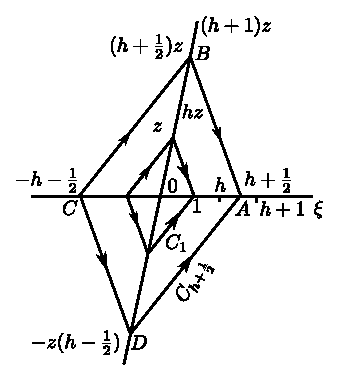
\includegraphics{fig2.eps}

\medskip
\centerline{\bf Fig.~2}
\end{figure}

Let\pageoriginale us consider the integral
$$
\frac{1}{8}\int_{C_{t}}\cot \pi\zeta\cot \frac{\pi
  \zeta}{z}\frac{d\zeta}{\zeta}
$$
where $C_{t}$ is the contour of the parallelogram in the $\zeta$-plane
with vertices at $\zeta=t$, $tz$, $-t$ and $-tz$ ($t$ positive and not
integral).

The integrand is a meromorphic function of $\zeta$. It has simple
poles at $\zeta=\pm k$ and $\zeta=\pm kz(k=1,2,3,\ldots)$ with
residues $\dfrac{1}{\pi k}\cot \dfrac{\pi k}{z}$ and $\dfrac{1}{\pi
  k}\cot \pi kz$ respectively, as one can readily notice from the
expansion
$$
\cot \pi u=\frac{1}{\pi u}-\frac{\pi u}{3}+\cdots
$$
valid for $0<|u|<1$. Also, the integrand has a pole of the third order
at $\zeta=0$, with residue $-\frac{1}{3}(z+1/z)$.

Let $t=h+1/2$, $h$ being a positive integer. Then there are no poles
of the integrand on $C_{t}$ and inside $C_{t}$ there are poles at
$\zeta=0$, $\pm k$ and $\pm kz(k=1,2,\ldots,h)$. By Cauchy's theorem
on residues,
{\fontsize{9}{11}\selectfont
$$
\frac{1}{8}\int_{C_{h+\frac{1}{2}}}\cot\pi\zeta\cot\pi\frac{\zeta}{z}\frac{d\zeta}{\zeta}=\frac{2\pi
  i}{8}\left\{\mathop{{\sum}'}^{h}_{k=-h}\frac{1}{\pi k}\cot \frac{\pi
  k}{z}+\mathop{{\sum}'}^{h}_{k=-h}\frac{1}{\pi k}\cot \pi kz-\frac{1}{3}\left(z+\frac{1}{z}\right)\right\},
$$}\relax
the accent on $\Sigma$ indicating the omission of $k=0$ from the
summation. In other words,
\begin{equation*}
\frac{1}{8}\int_{C_{h+\frac{1}{2}}} \cot \pi \zeta \cot
\pi\frac{\zeta}{z} \frac{d\zeta}{\zeta} + \frac{\pi i}{12}
\left(z+\frac{1}{z}\right) = 
\frac{i}{2}\left\{\sum^{h}_{k=1}\frac{1}{k}\left(\cot  
\pi kz+\cot \frac{\pi k}{z}\right)\right\}.\tag{20}\label{20}
\end{equation*}

We wish to consider the limit of the relation \eqref{20} as $h$ tends
to infinity through the sequence of natural numbers.

For this purpose, let us first observe that if $\zeta=\xi+i\eta$, then
$$
\cot \pi \zeta=i\frac{e^{\pi i\zeta}+e^{-\pi i\zeta}}{e^{\pi
    i\zeta}-e^{-\pi i\zeta}}
$$
tends\pageoriginale to $-i$ if $\eta$ tends to $\infty$, and tends to
$+i$, if $\eta$ tends to $-\infty$. Similarly $\cot\pi(\zeta/z)$ tends
to $-i$, when the imaginary part of $\zeta/z$ tends to $\infty$ and to
$i$, when the latter tends to $-\infty$. If $O$ is the origin and
$\zeta$ tends to infinity along a ray $OP$ with $P$ on one of the open
segments $AB$, $BC$, $CD$, $DA$ of $C_{h+\frac{1}{2}}$ (see figure),
then $\cot \pi\zeta\cdot \pi(\zeta/z)$ tends to the values $+1$, $-1$,
$+1$, $-1$ respectively. Moreover, this process of tending to the
respective values is uniform, when the ray $OP$ lies between two fixed
rays from $O$, which lie in one of the sectors $AOB$, $BOC$, $COD$ or
$DOA$ and neither of which coincides with the lines $\eta=0$ or
$\zeta=\lambda z$ ($\lambda$ real). This means that the sequence of
functions $\{\cot \pi(h+1/2)\xi \cot\pi(h+1/2)(\zeta/z)\}$
$(h=1,2,\ldots)$ tends to the limits $+1$ or $-1$ uniformly on any
proper closed subsegment of a side of $C_{1}$.

Moreover, this sequence of functions is uniformly bounded on
$C_{1}$. This can be seen as follows. Let $K_{j}$ denote the discs
$|\zeta-j|<1/4$, $j=0$, $\pm 1$, $\pm 2,\ldots$. In view of the
periodicity of $\cot \pi \zeta$, let us confine ourselves to the
strip, $0\leq \xi\leq 2$. We then readily see that in the complement
of the set-union of the discs $K_{0}$, $K_{1}$ and $K_{2}$ with
respect to this vertical strip, the function $\cot \pi \zeta$ is
bounded; for $\cot\pi \zeta$ tends to $\pm i$ as $\eta$ tends to
$\pm\infty$ and is bounded away from its poles at $\zeta=0$, $1$ and
$2$. Indeed therefore, $\cot \pi \zeta$ is bounded in the complement
of the set union of the discs $K_{j}$, $j=0$, $\pm 1,\ldots$ with
respect to the entire plane. Since the contours $C_{h+\frac{1}{2}}$,
for $h=1,2,\ldots$ lie in the complement, we have $|\cot \pi
\zeta|\leq \alpha$ for $\zeta\in C_{h+\frac{1}{2}}$ and $\alpha$
independent of $h$ and $\zeta$. By a similar argument for $\cot(\pi
\zeta/z)$ concerning its poles at $\pm kz$, we see that for $\zeta\in
C_{h+\frac{1}{2}}$, $h=1,2,\ldots|\cot(\pi \zeta/z)|\leq \beta$,
$\beta$ independent of $h$ and $\zeta$. In other words, the sequence
of functions $\{\cot \pi(h+\frac{1}{2})\zeta\cot
\pi(h+\frac{1}{2})(\zeta/z)\}$ is uniformly bounded on $c_{1}$. Now
\begin{equation*}
\int_{C_{h+\frac{1}{2}}}\cot \pi\zeta\cot \frac{\pi
  \zeta}{z}\frac{d\zeta}{\zeta}=\int_{C_{1}}\cot\pi\left(h+\frac{1}{2}\right)\zeta\cot\pi\left(h+\frac{1}{2}\right)\frac{\zeta}{z}\frac{d\zeta}{\zeta},\tag{21}\label{21} 
\end{equation*}
and in view of the foregoing considerations, we can interchange the
passage to the limit (as $h$ tends to infinity) and the integration,
on the right side of \eqref{21}. Thus, letting $h$ tend to infinity,
we obtain from \eqref{20},
\begin{align*}
& \frac{\pi
  i}{12}\left(z+\frac{1}{z}\right)+\frac{1}{8}\left(\int^{z}_{1}-\int^{-1}_{z}+\int^{-z}_{-1}-\int^{1}_{-z}\right)\frac{d\zeta}{\zeta}\\
& =\frac{i}{2}\left\{\sum^{\infty}_{k=1}\frac{1}{k}\left(\cot\pi
  kz+\cot\frac{\pi k}{z}\right)\right\}.\tag{22}\label{22}
\end{align*}\pageoriginale
Now
$$
\frac{1}{8}\left(\int^{z}_{1}-\int^{-1}_{z}+\int^{-z}_{-1}-\int^{1}_{-z}\right)\frac{d\zeta}{\zeta}=\frac{1}{4}\left(\int^{z}_{1}+\int^{z}_{-1}\right)\frac{d\zeta}{\zeta}. 
$$
For $z$ in the $\zeta$-plane cut along the negative $\xi$-axis, let
$\log z$ denote the branch that is real on the positive
$\xi$-axis. Then we see
$$
\int^{z}_{1}\frac{d\zeta}{\zeta}=\log z\text{ \ and \ }
\int^{z}_{-1}\frac{d\zeta}{\zeta}=\log z-\pi i.
$$
Thus from \eqref{22},
\begin{equation*}
\frac{\pi i}{12}\left(z+\frac{1}{z}\right)+\frac{1}{2}\left(\log
z-\frac{\pi
  i}{2}\right)=\frac{i}{2}\left(\sum^{\infty}_{k=1}\frac{1}{k}\left(\cot
\pi kz+\cot \frac{\pi k}{z}\right)\right\}.\tag{23}\label{23}
\end{equation*}

We insert in \eqref{23}, the expansions
$$
\cot \pi kz=-i\left(1+2\frac{e^{2\pi ikz}}{1-e^{2\pi
    ikz}}\right)=-i\left(1+2\sum^{\infty}_{m=1}e^{2\pi imkz}\right)
$$
and
$$
\cot \frac{\pi k}{z}=i\left(1+2\frac{e^{-2\pi ik/z}}{1-e^{-2\pi
    ik/z}}\right)=i\left(1+2\sum^{\infty}_{m=1}e^{-2im\pi k/z}\right);
$$
then we see that the resulting double series is absolutely
convergent. We are therefore justified in summing over $k$ first; we
see as a result that the series \eqref{23} goes over into
$$
-\sum^{\infty}_{m=1}\log\frac{(1-e^{2\pi imz})}{(1-e^{-2\pi
    im/z})}=\log\frac{\eta\left(-\dfrac{1}{z}\right)}{\eta(z)}+\frac{\pi
  i}{12}\left(z+\frac{1}{z}\right).
$$
Finally
$$
\log\frac{\eta\left(-\frac{1}{z}\right)}{\eta(z)}=\frac{1}{2}\left(\log
z-\frac{\pi i}{2}\right)=\log\sqrt{\frac{z}{i}},
$$
where\pageoriginale $\sqrt{z/i}$ is that branch which takes the value
$1$ at $z=i$ \ie $\eta(-1/z)=\sqrt{(z/i)}\eta(z)$.

We wish to remark that it was only for the sake of simplicity that we
took a parallelogram $C_{1}$ and considered `dilatations'
$C_{h+\frac{1}{2}}$ of $C_{1}$. It is clear that instead of the
parallelogram, we could have taken any other closed contour passing
through $1$, $z$, $-1$, $-z$ and through no other poles of the
integrand and worked with corresponding `dilatations' of the same.

\section{The second limit formula of Kronecker}\label{chap1:sec3}

\textsc{We Shall} consider now some problems more general than the
ones concerning the analytic continuation of the function
$\zeta_{Q}(s)$ in the half-plane $\sigma>1/2$ and the Kronecker limit
formula for $\zeta_{Q}(s)$.

In the first place, we ask whether it is possible to continue
$\zeta_{Q}(s)$ analytically in a larger half-plane; this question
shall be postponed for the present. We shall show later
(\S\ \ref{chap1:sec5}) that $\zeta_{Q}(s)$ has an analytic continuation in
the entire plane which is regular except for the simple pole at $s=1$
and satisfies a functional equation similar to that of the Riemann
$\zeta$-function.

Instead of
$\zeta_{Q}(s)=\mathop{{\sum}'}\limits^{\infty}_{m,n=-\infty}(Q(m,n))^{-s}$,
one might also consider
$$
\sum^{\infty}_{m,n=-\infty}(Q(m+\mu,n+\nu))^{-s}
$$
where $\mu$ and $\nu$ are non-zero real numbers which are not both
integral and where $m$ and $n$ run independently from $-\infty$ to
$+\infty$. Or, instead of the positive-definite binary quadratic form
$Q(u,v)$, we might take a positive-definite quadratic form in more
than two variables. Let, in fact, $S=(s_{ij})$, $1\leq i$, $j\leq p$
be the matrix of a positive-definite quadratic form
$\sum\limits_{1\leq i,j\leq p}s_{ij}x_{i}x_{j}$ in $p$ variables. Let
us consider
$$
\zeta_{S}(s) = \sum^{\infty}_{x_{1},\ldots,x_{p} =
  -\infty}\left(\sum_{i,j}S_{ij}x_{i}x_{j}\right)^{-s}  
$$
$x_{1},\ldots,x_{p}$ running over all $p$-tuples of integers, except
$(0,\ldots,0)$. The function\pageoriginale $\zeta_{S}(s)$, known as
the Epstein zeta-function, is regular for $\sigma > p/2$. It was shown
by Epstein that $\zeta_{S}(s)$ can be continued analytically in the
entire $s$-plane, into a function regular except for a simple pole at
$s=p/2$ and satisfying the functional equation
$$
\pi^{-s}\Gamma(s)\zeta_{S}(s)=|S|^{-\frac{1}{2}}\pi^{-(p/2-s)}\Gamma\left(\frac{p}{2}-s\right)\zeta_{S^{-1}}\left(\frac{p}{2}-s\right)  
$$
Epstein also obtained for $\zeta_{S}(s)$, an analogue of the first
limit formula of Kronecker but this naturally involves more
complicated functions than $\eta(z)$.

We shall now consider a generalization of $\zeta_{Q}(s)$ which shall
lead us to the second limit formula of Kronecker. Namely, let $u$ and
$v$ be independent real parameters. Let, as before,
$Q(m,n)=am^{2}+2bmn+cn^{2}$ be a positive-definite binary quadratic
form and let $ac-b^{2}=1$, without loss of generality. We then define,
for $\sigma>1$,
\begin{equation*}
\zeta_{Q}(s,u,v)=\mathop{{\sum}'}_{m,n}e^{2\pi
  i(mu+nv)}(Q(m,n))^{-s}\tag{24}\label{24} 
\end{equation*}
$m$, $n$ running over all ordered pairs of integers except
$(0,0)$. The series converges absolutely for $\sigma>1$ and converges
uniformly in every half-plane $\sigma\geq
1+\epsilon(\epsilon>0)$. Thus $\zeta_{Q}(s,u,v)$ is a regular function
of $s$ for $\sigma>1$. If $u$ and $v$ are both integers, then
$\zeta_{Q}(s,u,v)=\zeta_{Q}(s)$ which has been already considered. We
shall, suppose, in the following, that
\begin{equation*}
u \text{ {\em and} } v \text{ {\em are not both integers.}}\tag{$\ast$}
\end{equation*}
Furthermore, on account of the periodicity of $\zeta_{Q}(s,u,v)$ in
$u$ and $v$, we can clearly suppose that $0\leq u$, $v<1$. The
condition $(\ast)$ then means that at least one of the two conditions
$0<u<1$, $0<v<1$ is satisfied. We might, without loss of generality,
suppose that $0<u<1$. For, otherwise, if $u=0$, then necessarily
$0<v<1$. In this case, let us take the positive-definite binary
quadratic form $Q_{1}(m,n)=cm^{2}+2bmn+an^{2}$; we see then that, for
$\sigma>1$, 
$$
\zeta_{Q}(s,u,v)=\mathop{{\sum}'}_{m,n}e^{2\pi 
  i(mv+nu)}(Q_{1}(m,n))^{-s}.
$$
And here, since $0<v<1$, $v$ shall play the role of $u$ in
\eqref{24}. 

We\pageoriginale shall prove now that $\zeta_{Q}(s,u,v)$ can be
continued analytically into a function regular in the half-plane
$\sigma>1/2$ and then determine its value at $s=1$; this will lead us
to the second limit formula of Kronecker.

For $\sigma>1$, by our earlier notation,
\begin{equation*}
\zeta_{Q}(s,u,v)=y^{s}\sum^{\infty}_{m=-\infty}e^{2\pi
  imu}|m|^{-2s} + y^{s}{\sum'}^{\infty}_{n=-\infty}e^{2\pi
  inv}\sum^{\infty}_{m=-\infty}e^{2\pi imu}|m+nz|^{-2s}.\tag{25}\label{25}
\end{equation*}

The first series in \eqref{25} converges absolutely for $\sigma>1/2$
and uniformly in every compact subset of this half-plane. Hence it
defines a regular function of $s$ for $\sigma>1/2$. The double series
in \eqref{25} again defines a regular function of $s$ in the
half-plane $\sigma>1$. To obtain its analytic continuation in a larger
half-plane, we shall carry out the summation of the double series in
the following particular way. Namely, we consider the finite partial
sums
$$
\mathop{{\sum}'}_{n_{1}\leq n\leq n_{2}}\sum_{m_{1}\leq m\leq
  m_{2}}e^{2\pi i(mu+nv)}|m+nz|^{-2s}.
$$
We shall show that when $m_{1}$ and $n_{1}$ tend to $-\infty$
independently and $m_{2}$ and $n_{2}$ tend to $\infty$ independently,
then these partial sums which are entire functions of $s$ converge
uniformly in every compact subset of the half-plane $\sigma>1/2$. The
proof is based on the method of partial summation in Abel's Theorem.

Let us define for any integer $k$, $c_{k}=\dfrac{e^{2\pi iku}}{e^{2\pi
    iu}-1}$. (Recall that $0<u<1$). Then $e^{2\pi
  imu}=c_{m+1}-c_{m}$. Moreover,
$$
|c_{m}|\leq |1-e^{2\pi iu}|^{-1}=\alpha,
$$
where $\alpha$ is independent of $m$. Now
\begin{align*}
& \mathop{{\sum}'}_{n_{1}\leq n\leq n_{2}}\sum_{m_{1}\leq m\leq
  m_{2}}e^{2\pi i(mu+nv)}|m+nz|^{-2s}\\
&= \mathop{{\sum}'}^{n_{2}}_{n=n_{1}}e^{2\pi
    inv}\sum^{m_{2}}_{m=m_{1}}\frac{c_{m+1}-c_{m}}{|m+nz|^{2s}}\\
&= \mathop{{\sum}'}^{n_{2}}_{n=n_{1}}e^{2\pi
    inv}\left(\sum^{m_{2}}_{m=m_{1}+1}c_{m}(|m-1+nz|^{-2s}-|m+nz|^{-2s})+\right.\\
&\qquad
  \left.\phantom{\sum^{m_{2}}_{m=m_{1}+1}}+c_{m_{2}+1}|m_{2}+nz|^{-2s}-c_{m_{1}}|m_{1}+nz|^{-2s}\right).\tag{26}\label{26} 
\end{align*}\pageoriginale
Let us also observe that
$$
\left|c_{m_{2}+1}|m_{2}+nz|^{-2s}\right|\leq
\alpha|n|^{-2\sigma}y^{-2\sigma}
$$
and
$$
\left|c_{m_{1}}|m_{1}+nz|^{-2s}\right|\leq
\alpha|n|^{-2\sigma}y^{-2\sigma}. 
$$
Further
\begin{align*}
& |\; | m-1+nz|^{-2s}-|m+nz|^{-2s}|\\
&\quad
= \left|-2s\int^{m}_{m-1}((\mu+nx)^{2}+n^{2}y^{2})^{-s-1}(\mu+nx)d\mu\right|\\
&\qquad \leq
2|s|\int^{m}_{m-1}((\mu+nx)^{2}+n^{2}y^{2})^{-(\sigma+\frac{1}{2})}d \mu. 
\end{align*}
Thus \eqref{26} is majorised by
\begin{equation*}
2|s|\alpha
\mathop{{\sum}'}^{n_{2}}_{n=n_{1}}\sum^{m_{2}}_{m=m_{1}+1}\int^{m}_{m-1}((\mu+nx)^{2}+n^{2}y^{2})^{-(\sigma+\frac{1}{2})}d\mu+2\alpha 
y^{-2\sigma}\mathop{{\sum}'}^{n_{2}}_{n=n_{1}}|n|^{-2\sigma}.\tag{27}\label{27} 
\end{equation*}
In \eqref{27}, we sum $m$ from $-\infty$ to $+\infty$ instead of
summing from $m_{1}+1$ to $m_{2}$ and then we see that \eqref{26} has
the majorant
$$
2\alpha|s|\mathop{{\sum}'}^{n_{2}}_{n=n_{1}}\int^{\infty}_{-\infty}((\mu+nx)^{2}+n^{2}y^{2})^{-(\sigma+\frac{1}{2})}d\mu+2\alpha
y^{-2\sigma}\sum^{n_{2}}_{n=n_{1}}|n|^{-2\sigma}. 
$$
Now\pageoriginale
\begin{align*}
\int^{\infty}_{-\infty}((\mu+nx)^{2}+n^{2}y^{2})^{-(\sigma+\frac{1}{2})}d\mu
&=
\int^{\infty}_{-\infty}(\mu^{2}+n^{2}y^{2})^{-(\sigma+\frac{1}{2})}d\mu\\
&=
|n|^{-2\sigma}y^{-2\sigma}\int^{\infty}_{-\infty}(1+\mu^{2})^{-(\sigma+\frac{1}{2})}d\mu.\tag{28}\label{28} 
\end{align*}
Since the integral in \eqref{28} converges for $\sigma>1/2$, we see
that \eqref{26} is majorised by
$\beta\mathop{{\sum}'}\limits^{n_{2}}_{n=n_{1}}|n|^{-2\sigma}$, $\beta$ depending
only on the compact set in which $s$ lies in the half-plane
$\sigma>1/2$ and on $\alpha$ and $y$.

If, in \eqref{26}, we now carry out the passage of $m_{1}$ and $n_{1}$
to $-\infty$ and of $m_{2}$ and $n_{2}$ to $+\infty$ independently,
then we see that the double series in \eqref{25} summed in this
particular manner, is majorised by the series $2\beta
\sum\limits^{\infty}_{n=1}n^{-2\sigma}$. Hence it converges uniformly
when $s$ lies in a compact set in the half-plane $\sigma>1/2$. Since
each partial sum \eqref{26} is an entire function of $s$, we see, by
Weierstrass' Theorem that the double series in \eqref{25} converges
uniformly to a function which is regular for $\sigma>1/2$ and which
provides the necessary analytic continuation in this half-plane.

Thus under the assumption that $u$ and $v$ are not both integers,
$\zeta_{Q}(s,\break u,v)$ has an analytic continuation which is regular for
$\sigma>1/2$. We shall now determine its value at $s=1$. We wish to
make it explicit that hereafter we shall make only the assumption
$(\ast)$ and not the specific assumption $0<u<1$.

From the convergence proved above, it follows that
\begin{align*}
\zeta_{Q}(1,u,v) &=
\frac{z-\ob{z}}{2i}\mathop{{\sum}'}^{\infty}_{m=-\infty}\frac{e^{2\pi
    imu}}{|m|^{2}}+\\ 
&\quad
+\frac{z-\ob{z}}{2i}\mathop{{\sum}'}^{\infty}_{n=-\infty}e^{2\pi
  inv}\sum^{\infty}_{m=-\infty}\frac{e^{2\pi
    imu}}{(m+nz)(m+n\ob{z})}\tag{29}\label{29} 
\end{align*} 
where the accents on $\Sigma$ have the usual meaning.

In order to sum $\sum\limits^{\infty}_{m=-\infty}\frac{e^{2\pi
    imu}}{|m|^{2}}$, we observe that since the series
$$\sum\limits^{\infty}_{m=-\infty}\frac{e^{2\pi
    imu}}{m}$$\pageoriginale 
converges uniformly to $2\pi(1/2-u)$ in
any closed interval. $0<p\leq u\leq q<1$, we have
\begin{align*}
\int^{u}_{0}\left(\mathop{{\sum}'}^{\infty}_{m=-\infty}\frac{e^{2\pi
    imu}}{m}\right)du &= \lim\limits_{\epsilon\to
  0}\int^{u}_{\epsilon}\left(\mathop{{\sum}'}^{\infty}_{m=-\infty}\frac{e^{2\pi
    imu}}{m}\right)du\\
&= \lim\limits_{\epsilon\to
  0}\mathop{{\sum}'}^{\infty}_{m=-\infty}\int^{u}_{\epsilon}\frac{e^{2\pi
    imu}}{m}du, 
\end{align*}
\ie
$$
2\pi i(u-u^{2})=\frac{1}{2\pi i}\lim\limits_{\epsilon\to
  0}\left(\mathop{{\sum}'}^{\infty}_{m=-\infty}\frac{e^{2\pi
    imu}}{m^{2}}-\mathop{{\sum}'}^{\infty}_{m=-\infty}\frac{e^{2\pi
    imu}}{m^{2}}\right),
$$
\ie
$$
2\pi^{2}(u^{2}-u)=\mathop{{\sum}'}^{\infty}_{m=-\infty}-\frac{e^{2\pi
    imu}}{m^{2}}-\frac{\pi^{2}}{3}, 
$$
since $\mathop{{\sum}'}\limits^{\infty}_{m=-\infty}\dfrac{e^{2\pi
    imu}}{m^{2}}$ is continuous in $u$. In other words,
$$
\mathop{{\sum}'}^{\infty}_{m=-\infty}\frac{e^{2\pi
    imu}}{m^{2}}=2\pi^{2}\left(u^{2}-u+\frac{1}{6}\right). 
$$

We shall sum the double series in \eqref{29} more generally with
$\ob{z}$ replaced by $r$, where $-r\in\mathfrak{H}$. Leter, we shall
set $r=\ob{z}$. We remark that with slight changes, our arguments
concerning the series $\sum' e^{2\pi i(mu+nv)}|\break m+nz|^{-2s}$ above will
also go through for the double series $\sum' e^{2\pi
  i(mu+nv)}\break ((m+nz)\cdot (m+nr))^{-s}$. Now for summing the series
\begin{align*}
& \frac{z-r}{2i}\mathop{{\sum}'}^{\infty}_{n=-\infty}e^{2\pi
  inv}\sum^{\infty}_{m=-\infty}\frac{e^{2\pi imu}}{(m+nz)(m+nr)}\\
& =\frac{1}{2i}\mathop{{\sum}'}^{\infty}_{n=-\infty}\frac{e^{2\pi
      inv}}{n}\sum^{\infty}_{m=-\infty}e^{2\pi
    imu}\left(\frac{1}{m+nr}-\frac{1}{m+nz}\right).\tag{30}\label{30} 
\end{align*}
we could apply the Poisson summation formula with respect to $m$ to
the inner sum on the left side of \eqref{30}, but we shall adopt a
different method here. 

Let\pageoriginale us define, for complex $z=x+iy$,
$$
f(z)=\frac{1}{z} + \sum^{\infty}_{m=1}\left(\frac{e^{2\pi
    imu}}{z+m}+\frac{e^{-2\pi imu}}{z-m}\right)
$$
and consider $f(z)$ in the strip $-1/2\leq x\leq 1/2$. It is not hard
to see that whenever $z$ lies in a compact set not containing $z=0$ in
this strip, the series converges uniformly and hence $f(z)$ is regular
in this strip except at $z=0$, where it has a simple pole with residue
$1$. Moreover, one can show that $f(z)-1/z$ is bounded in this
strip. Further
$$
f(z+1)=e^{-2\pi iu}f(z).
$$

Consider now the function
$$
g(z)=2\pi i\frac{e^{-2\pi iuz}}{1-e^{-2\pi iz}};
$$
$g(z)$ is again regular in this strip except at $z=0$ where it has a
simple pole with residue $1$. Moreover $g(z) - 1/z$ is bounded in this
strip; as a matter of fact, if $0<u<1$, $g(z)$ tends to $0$ if $y$
tends to $+\infty$ or $-\infty$ and if $u=0$, then $g(z)$ tends to $0$
or $2\pi i$ according as $y$ tends to $+\infty$ or $-\infty$. Further
$g(z+1)=e^{-2\pi iu}g(z)$.

As a consequence, the function $f(z)-g(z)$ is regular and bounded in
this strip and since $f(z+1)-g(z+1)=e^{-2\pi iu}(f(z)-g(z))$, it is
regular in the whole $z$-plane and bounded, too. By Liouville's
theorem, $f(z)-g(z)=c$, a constant. It can be seen that, if $u\neq 0$,
$c=0$ and if $u=0$, $c=\pi i$, by using the series expansion for the
function $\pi\cot \pi z$. In any case,
\begin{equation*}
f(nr)-f(nz)=g(nr)-g(nz).\tag{31}\label{31}
\end{equation*}

In view of the convergence-process of the series \eqref{29} described\break
above, we can rewrite the double series \eqref{30} as
{\fontsize{9}{11}\selectfont
\begin{align*}
& \frac{1}{2i}\mathop{{\sum}'}^{\infty}_{n=-\infty}\frac{e^{2\pi
    inv}}{n}\left\{\frac{1}{nr}-\frac{1}{nz}+\sum^{\infty}_{m=1}e^{2\pi
  imu}\left(\frac{1}{m+nr}+\frac{1}{-m+nr}-\frac{1}{m+nz}-\frac{1}{-m+hz}\right)\right\}\\
& =\frac{1}{2i}\mathop{{\sum}'}^{\infty}_{n=-\infty}\frac{e^{2\pi
      inv}}{n}(f(nr)-f(nz))=\pi
  \mathop{{\sum}'}^{\infty}_{n=-\infty}\frac{e^{2\pi
      inv}}{n}\left(\frac{e^{-2\pi iunr}}{1-e^{-2\pi
      inr}}-\frac{e^{-2\pi iunz}}{1-e^{-2\pi
      inz}}\right),\tag{32}\label{32}
\end{align*}}\pageoriginale
by \eqref{31}. Now, we insert in \eqref{32}, the expansions
\begin{align*}\relax
(1-e^{-2\pi inz})^{-1} &=
\begin{cases}
-\sum^{\infty}_{m=1}e^{2\pi imnz}, & (n>0)\\
\sum^{\infty}_{m=0}e^{-2\pi imnz}, & (n<0)
\end{cases}\\
(1-e^{-2\pi inr})^{-1} &= 
\begin{cases}
\sum^{\infty}_{m=0}e^{-2\pi imnr}, & (n>0)\\
-\sum^{\infty}_{m=1}e^{2\pi imnr}, & (n<0)
\end{cases}
\end{align*}
valid for $z$, $-r\in \mathfrak{H}$ and then the series \eqref{32}
goes over into 
\begin{align*}
& \pi \sum^{\infty}_{n=1}\frac{1}{n}\left\{e^{2\pi in(v-ur)}+e^{-2\pi
  in(v-uz)}+\sum^{\infty}_{m=1}(e^{-2\pi in(v-uz-mz)}+\right.\\
& \qquad \left. \phantom{\sum^{\infty}_{m=1}} +e^{2\pi in(v-ur-mr)}+e^{2\pi
  in(v-uz+m z)}+e^{-2\pi in(v-ur+mr)})\right\}\tag{33}\label{33}
\end{align*}
If $0<u<1$, then this series converges absolutely, since $z$, $-r\in
\mathfrak{H}$. Carrying out the summation over $n$ first, we see that
this double series is equal to
\begin{align*}
& -\pi\log\left\{\prod^{\infty}_{m=0}(1-e^{-2\pi
    i(v-uz-mz)})(1-e^{2\pi i(v-ur-mr)})\times\right.\\
&\qquad \left. \times\prod^{\infty}_{m=1}(1-e^{2\pi
    i(v-uz+mz)})(1-e^{-2\pi i(v-ur+mr)})\right\}.\tag{34}\label{34}
\end{align*}
If $u=0$, then necessarily $0<v<1$ and in this case,
$$
\pi \sum^{\infty}_{n=1}\frac{1}{n}(e^{2\pi inv}+e^{-2\pi
  inv})=-\pi\log(1-e^{2\pi iv})(1-e^{-2\pi iv}). 
$$
The\pageoriginale rest of the series \eqref{33} is absolutely
convergent and summing over $n$ first, we see that the value of the
series \eqref{33} is given by the expression \eqref{34}.

Let us now set $v-uz=w$, $v-ur=q$. Then replacing $\ob{z}$ by $r$ in
\eqref{29}, we have finally, for $0\leq u$, $v<1$ and $u$ and $v$ not
simultaneously zero,
\begin{align*}
& \frac{z-r}{2i}\sum^{\infty}_{m,n=-\infty}\frac{e^{2\pi
      i(mu+nv)}}{(m+nz)(m+nr)}\\
&= -\pi^{2}i(z-r)\left(u^{2}-u+\frac{1}{6}\right)-\pi
  \log\left\{\prod^{\infty}_{m=0}(1-e^{-2\pi i(w-mz)})\times\right.\\
&\qquad \left.\times (1-e^{2\pi i(q-mr)})\times
  \prod^{\infty}_{m=1}(1-e^{2\pi i(w+mz)})(1-e^{-2\pi
    i(q+mr)})\right\}\tag{35}\label{35} 
\end{align*}

For $z\in \mathfrak{H}$ and arbitrary complex $w$, the elliptic
theta-function\break $\vartheta_{1}(w,z)$ is defined by the infinite series,
$$
\vartheta_{1}(w,z)=\sum^{\infty}_{n=-\infty}e^{\pi
  i(n+\frac{1}{2})^{2}z+2\pi i(n+\frac{1}{2})(w-\frac{1}{2})}.
$$
It is clear that this series converges absolutely, uniformly when $z$
lies in a compact set in $\mathfrak{H}$ and $w$ in a compact set of
the $w$-plane. Hence $\vartheta_{1}(w,z)$ is an analytic function of
$z$ and $w$ for $z\in\mathfrak{H}$ and complex $w$. It is proved in
the theory of the elliptic theta-functions that $\vartheta_{1}(w,z)$
can also be expressed as an absolutely convergent infinite product,
namely,
\begin{align*}
\vartheta_{1}(w,z) &= -ie^{\pi i(z/4)}(e^{\pi iw}-e^{-\pi iw})\times\\
&\quad \times\prod^{\infty}_{m=1}(1-e^{2\pi i(w+mz)})(1-e^{-2\pi
  i(w-mz)})(1-e^{2\pi imz}).\tag{36}\label{36}
\end{align*}
We shall identify these two forms of $\vartheta_{1}(w,z)$ later
on. For the present, we shall consider $\vartheta_{1}(w,z)$ as defined
by the infinite product.

Now a simple rearrangement of the expression \eqref{35} gives
\begin{align*}
& \frac{z-r}{2i}\mathop{{\sum}'}^{\infty}_{m,n=-\infty}\frac{e^{2\pi
    i(mu+nv)}}{(m+nz)(m+nr)}\\
&\quad
  =-\pi^{2}i(z-r)\left(u^{2}-u+\frac{1}{6}\right)+\pi^{2}i\left((w-q)+\frac{1}{6}(z-r)\right)-\\
&\qquad -\pi
  \log\frac{\vartheta_{1}(w,q)\vartheta_{1}(q,-r)}{\eta(z)\eta(-r)}\\
&\quad = -\pi^{2}i\frac{(w-q)^{2}}{z-r}-\pi
  \log\frac{\vartheta_{1}(w,q)\vartheta_{1}(q,-r)}{\eta(z)\eta(-r)}\\
&\frac{z-r}{-2\pi i}\mathop{{\sum}'}_{m,n}\frac{e^{2\pi
      i(mu+nv)}}{(m+nz)(m+nr)}=\log
  \frac{\vartheta_{1}(w,z)\vartheta_{1}(q,-r)}{\eta(z)\eta(-r)}e^{\pi i((w-q)^{2}/(z-r))}.\tag{37}\label{37}
\end{align*}\pageoriginale
Setting $r=\ob{z}$ again, we have $q=\ob{w}$ and then
$$
\zeta_{Q}(1,u,v)=-\pi^{2}i\frac{(w-\ob{w})^{2}}{z-\ob{z}}-\pi
\log\frac{\vartheta_{1}(w,z)\vartheta_{1}(\ob{w},-\ob{z})}{|\eta(z)|^{2}}
$$
One can see easily from \eqref{36} that
$\ob{\vartheta_{1}(w,z)}=\vartheta_{1}(\ob{w},-\ob{z})$. Hence
\begin{equation*}
\zeta_{Q}(1,u,v)=-\pi^{2}iu^{2}(z-r)-2\pi
\log\left|\frac{\vartheta_{1}(w,z)}{\eta(z)}\right|,\tag{38}\label{38} 
\end{equation*}
for $0\leq u$, $v<1$ and $u$ and $v$ not both zero.

We contend that formula \eqref{38} is valid for all $u$ and $v$ not
both integral. Since
$\zeta_{Q}(1,u+1,v)=\zeta_{Q}(1,u,v+1)=\zeta_{Q}(1,u,v)$ and $w$ goes
over into $w+1$ and $w-z$ respectively under the transformations $v\to
v+1$ and $u\to u+1$, it would suffice for this purpose to prove that
$$
\zeta_{Q}(1,u,v)=-\pi^{2}iu^{2}(z-r)-2\pi
\log\left|\frac{\vartheta_{1}(w+1,z)}{\eta(z)}\right|
$$
and
$$
\zeta_{Q}(1,u,v)=-\pi^{2}i(u+1)^{2}(z-r)-2\pi \log
\left|\frac{\vartheta_{1}(w-z,z)}{\eta(z)}\right|. 
$$
The first assertion is an immediate consequence of the fact that
$\vartheta_{1}(w+1,z)=-\vartheta_{1}(w,z)$. To prove the second, we
observe that from \eqref{36}, we have 
\begin{align*}
\frac{\vartheta_{1}(w-z,z)}{\vartheta_{1}(w,z)} &= \frac{(e^{\pi i(w-z)}-e^{-\pi i(w-z)})(1-e^{2\pi iw})}{(e^{\pi iw}-e^{-\pi iw})(1-e^{-2\pi i(w-z)})}\\
&= e^{+2\pi iw-\pi iz}
\end{align*}\pageoriginale
and hence
\begin{align*}
2\pi\left(\log\left|\frac{\vartheta_{1}(w-z,z)}{\eta(z)}\right|-\log\left|\frac{\vartheta_{1}(w,z)}{\eta(z)}\right|\right) &= +\pi^{2}i\{(2(w-\ob{w})-(z-\ob{z})\}\\
&= -\pi^{2}i(z-\ob{z})((u+1)^{2}-u^{2}).
\end{align*}
Thus the second assertion is proved and we have

\begin{thm}\label{chap1:thm2}
If $u$ and $v$ are real and not both integral, then the Epstein
zeta-function $\zeta_{Q}(s,u,v)$ defined by \eqref{24} for $\sigma>1$,
can be continued analytically into a function regular for $\sigma>1/2$
and its value at $s=1$ is given by \eqref{38}. 
\end{thm}

We are finally led to the following formula: viz.\@ {\em for all $u$
  and $v$ not both integral},
$$
\frac{z-\ob{z}}{2i}\mathop{{\sum}'}_{m,n}\frac{e^{2\pi
    i(mu+nv)}}{|m+nz|^{2}}=-\pi^{2}i\frac{(w-\ob{w})^{2}}{z-\ob{z}}-2\pi
\log \left|\frac{\vartheta_{1}(w,z)}{\eta(z)}\right|.
$$
This is the second limit formula of Kronecker. We may rewrite it as
\begin{equation*}
\frac{z-\ob{z}}{-2\pi i}\sum'\frac{e^{2\pi i(mu+nv)}}{|m+nz|^{2}}=\log
\left|\frac{\vartheta_{1}(v-uz,z)}{\eta(z)}e^{\pi
  izu^{2}}\right|^{2}.\tag{39}\label{39} 
\end{equation*}

If $u$ and $v$ are both integral, then $v-uz$ is a zero of
$\vartheta_{1}(w,z)$ and then both sides are infinite.

\section{The elliptic theta-function $\vartheta_{1}(w,z)$}\label{chap1:sec4}

For $z=x+iy\in\mathfrak{H}$ and arbitrary complex $w$, the elliptic
theta-function $\vartheta_{1}(w,z)$ was defined in \S\ \ref{chap1:sec3}, by
the infinite product \eqref{36}. $\vartheta_{1}(w,z)$ is a regular
function of $z$ and $w$, for $z$ in $\mathfrak{H}$ and arbitrary
complex $w$. We shall now develop the transformation-theory of
$\vartheta_{1}(w,z)$ under modular transformations, as a consequence
of the second limit formula of Kronecker.

Let\pageoriginale $u$ and $v$ be arbitrary real numbers which are not
simultaneously integral. Let $z\to z^{\ast}=(\alpha z+\beta)(\gamma
z+\delta)^{-1}=x^{\ast}+iy^{\ast}$ be a modular transformation. Then
$u^{\ast}=\delta u+\gamma v$ and $v^{\ast}=\beta u+\alpha v$ are again
real numbers, which are not both integral. For $\sigma>1$, we have
\begin{align*}
y^{\ast s}\sum^{\infty}_{m,n=-\infty}\frac{e^{2\pi
    i(mu^{\ast}+nv^{\ast})}}{|m+nz^{\ast}|^{2s}} &=
  y^{s}\mathop{{\sum}'}_{m,n}\frac{e^{2\pi
      i((m\delta+n\beta)u+(m\gamma+n\alpha)v)}}{|(m\delta+n\beta)+(m\gamma+n\alpha)z|^{2s}}\\
&= y^{s}\mathop{{\sum}'}_{m,n}\frac{e^{2\pi i(mu+nv)}}{|m+nz|^{2s}}.
\end{align*}
From \S\ \ref{chap1:sec3}, we know that both sides, as functions of $s$,
have analytic continuations regula in the half-plane $\sigma>1/2$ and
hence the equality of the two sides is valid even for $\sigma>1/2$. In
particular, for $s=1$,
\begin{equation*}
y^{\ast}\mathop{{\sum}'}_{m,n}\frac{e^{2\pi
    i(mu^{\ast}+nv^{\ast})}}{|m+nz^{\ast}|^{2}}=y\mathop{{\sum}'}_{m,n}\frac{e^{2\pi
    i(mu+nv)}}{|m+nz|^{2}}.\tag{40}\label{40}
\end{equation*}
By Kronecker's second limit formula,
$$
-\pi^{2}i\frac{(w^{\ast}-\ob{w}^{\ast})^{2}}{z^{\ast}-\ob{z}^{\ast}}-2\pi\log
\left|\frac{\vartheta_{1}(w^{\ast},z^{\ast})}{\eta(z^{\ast})}\right|=-\pi^2
i\frac{(w-\ob{w})^{2}}{z-\ob{z}}-2\pi 
\log\left|\frac{\vartheta_{1}(w,z)}{\eta(z)}\right| 
$$
where $w=v-uz$ and $w^{\ast}=v^{\ast}-u^{\ast}z^{\ast}=w/(\gamma
z+\delta)$. Therefore,
\begin{align*}
&
  \log\left|\frac{\vartheta_{1}(w^{\ast},
z^{\ast})}{\eta(z^{\ast})}\right| -
  \log\left|\frac{\vartheta_{1}(w,z)}{\eta(z)}\right|  
  =\frac{\pi 
  i}{2}\frac{(w - \ob{w})^{2}}{z-\ob{z}}-\frac{\pi
  i}{2}\frac{(w^{\ast}-\ob{w}^{\ast})^{2}}{z^{\ast}-\ob{z}^{\ast}}\\
&=\frac{\pi i\gamma}{2}\left(\frac{w^{2}}{\gamma
    z+\delta}-\frac{\ob{w}^{2}}{\gamma\ob{z}+\delta}\right)=\log\left|e^{(\pi
    i\gamma w^{2})/(\gamma z+\delta)}\right|  
\end{align*}
Thus
\begin{equation*}
\frac{\vartheta_{1}\left(\frac{w}{\gamma z+\delta}, \frac{\alpha
    z+\beta}{\gamma z+\delta}\right)}{\eta\left(\frac{\alpha
    z+\beta}{\gamma
    z+\delta}\right)}=\frac{\vartheta_{1}(w,z)}{\eta(z)}e^{(\pi
  i\gamma w^{2})/(\gamma z+\delta)}\cdot \omega,\tag{41}\label{41}
\end{equation*}
where $|\omega|=1$ and $\omega$ might depend on every one of $w$, $z$,
$\alpha$, $\beta$, $\gamma$ and $\delta$. But\pageoriginale from
\eqref{41}, we observe that $\omega$ is a regular function of $z$ in
$\mathfrak{H}$ and $w$, except possibly when $w$ is of the form $m+nz$
with integral $m$ and $n$. But since $|\omega|=1$, we see, by applying
the maximum modulus principle to $\omega$ as a function of $w$ and of
$z$, that $\omega$ is independent of $w$ and $z$. Hence
$\omega=\omega(\alpha,\beta,\gamma,\delta)$. 

Now from the fact that
$$
\vartheta_{1}(w,z)=2\pi \eta^{3}(z)w+\cdots
$$
we note that $\vartheta'_{1}(0,z)$, the value of the derivative of
$\vartheta_{1}(w,z)$ with respect to $w$ at $w=0$, is equal to $2\pi
\eta^{3}(z)$. Differentiating the relation \eqref{41} with respect to
$w$ at $w=0$, we get
$$
\frac{1}{\gamma z+\delta}\frac{\vartheta'_{1}\left(0,\frac{\alpha
    z+\beta}{\gamma z+\delta}\right)}{\eta\left(\frac{\alpha
    z+\beta}{\gamma
    z+\delta}\right)}=\frac{\vartheta'_{1}(0,z)}{\eta(z)}\omega, 
$$
\ie
$$
(\gamma z+\delta)^{-1}\eta^{2}\left(\frac{\alpha z+\beta}{\gamma
  z+\delta}\right)=\omega\eta^{2}(z). 
$$

We have thus rediscovered the formula
$$
\eta\left(\frac{\alpha z+\beta}{\gamma
  z+\delta}\right)=\epsilon\sqrt{\gamma z+\delta}\eta(z)
$$
with $\epsilon$ being a $24^{\text{th}}$ root of unity depending only
on $\alpha$, $\beta$, $\gamma$ and $\delta$ and
$\omega=\epsilon^{2}$. Rewriting \eqref{41}, we obtain

\begin{proposition}\label{prop4}
The elliptic theta-function has the transformation formula
$$
\vartheta_{1}\left(\frac{w}{\gamma z+\delta},\frac{\alpha
  z+\beta}{\gamma z+\delta}\right)=\epsilon^{3}\sqrt{\gamma
  z+\delta}e^{(\pi i\gamma w^{2})/(\gamma z+\delta)}\vartheta_{1}(w,z) 
$$
under a modular substitution $z\to(\alpha z+\beta)(\gamma
z+\delta)^{-1}$, $\epsilon^{3}$ being an $8^{\text{th}}$ root of unity
depending only on $\alpha$, $\beta$, $\gamma$ and $\delta$.
\end{proposition}

From the transformation-theory of $\eta(z)$ we know that corresponding
to the modular transformations $z\to z+1$ and $z\to -1/z$,
$\epsilon^{3}$ has respectively the values $e^{\pi i/4}$ and $e^{-3\pi
  i/4}$. Hence 
\begin{equation*}
\left.
\begin{aligned}
\vartheta_{1}(w,z+1) &= e^{\pi i/4}\vartheta_{1}(w,z)\\
\vartheta_{1}\left(\frac{w}{z},-\frac{1}{z}\right) &= e^{\pi
  iw^{2}/z}\frac{1}{i}\sqrt{\frac{z}{i}}\vartheta_{1}(w,z). 
\end{aligned}\right\}
\tag{42}\label{42}
\end{equation*}\pageoriginale
Once again using the fact that the modular transformations $z\to z+1$
and $z\to -1/z$ generate the elliptic modular group, we can determine
$\epsilon^{3}$, with the help of \eqref{42}, by a process of
`reduction'. Hermite found an explicit expression for $\epsilon^{3}$,
involving the well-known Gaussian sums.

We now wish to make another remark which is of function-theoretic
significance and which is again, a consequence of Kronecker's second
limit formula.

Let us define for $z\in\mathfrak{H}$ and real $u$ and $v$ (not both
integral), the function
$$
f(z,u,v)=\log\left(\frac{\vartheta_{1}(v-uz,z)}{\eta(z)}e^{\pi izu^{2}}\right)
$$
choosing a fixed branch of the logarithm in $\mathfrak{H}$. Then from
\eqref{40} and \eqref{39},
$$
\log\left|\frac{\vartheta_{1}(v^{\ast}-u^{\ast}z^{\ast},z^{\ast})}{\eta(z^{\ast})}e^{\pi
  iz^{\ast}u^{\ast
    2}}\right|=\log\left|\frac{\vartheta_{1}(v-uz,z)}{\eta(z)}e^{\pi
  izu^{2}}\right|. 
$$
Hence
$$
f\left(\frac{\alpha z+\beta}{\gamma z+\delta}, \delta u+\gamma v,
\beta u+\alpha v\right)=f(z,u,v)+i\lambda,
$$
where $\lambda$ is real and might depend on $z$, $u$, $v$, $\alpha$,
$\beta$, $\gamma$ and $\delta$. But since $\lambda$ is a regular
function of $z$, whose imaginary part is zero in $\mathfrak{H}$,
$\lambda$ is independent of $z$. Thus
\begin{equation*}
f\left(\frac{\alpha z+\beta}{\gamma z+\delta},\delta u+\gamma v,\beta
u+\alpha
v\right)=f(z,u,v)+i\lambda(u,v,\alpha,\beta,\gamma,\delta).\tag{43}\label{43} 
\end{equation*}

Let now $q>1$, be a fixed integer and let $u$ and $v$ be proper
rational fractions with reduced denominator $q$ \ie $u=a/q$, $v=a/q$,
$(a,b,q)=1$ and $0\leq u$, $v<1$. Since $\alpha\delta-\beta\gamma=1$,
we have again.
$$
(\delta a+\gamma b, \beta a+\alpha b,q)=1.
$$

Now\pageoriginale from \eqref{39}, we see that
$\log\left|\dfrac{\vartheta_{1}(v-uz,z)}{\eta(z)}e^{\pi
  izu^{2}}\right|$ is invariant under the transformations $u\to u+1$
and $v\to v+1$. Hence $f(z,u,v)$ picks up a purely imaginary additive
constant under these transformations. If now, $(\delta a+\gamma
b)/q\equiv (a^{\ast}/q)(\mod 1)$ and $(\beta a+\alpha b)/q\equiv
(b^{\ast}/q)(\mod 1)$ where $a^{\ast}/q$, $b^{\ast}/q$ are proper
rational fractions with reduced denominator $q$, then
$$
f\left(\frac{\alpha z+\beta}{\gamma z+\delta}, \frac{\delta a+\gamma
  b}{q},\frac{\beta a+\gamma b}{q}\right)=f\left(\frac{\alpha
  z+\beta}{\gamma z+\delta},
\frac{a^{\ast}}{q},\frac{b^{\ast}}{q}\right)+i\lambda' 
$$
where $\lambda'$ is real and depends on $a$, $b$, $\alpha$, $\beta$,
$\gamma$ and $\delta$. Writing $f(z,a/q,b/q)$ as $f_{a,b}(z)$, we get
from \eqref{43},
\begin{equation*}
f_{a^{\ast},b^{\ast}}\left(\frac{\alpha z+\beta}{\gamma
  z+\delta}\right)=f_{a,b}(z)+i\lambda^{\ast}(a,b,\alpha,\beta,\gamma,\delta)\tag{44}\label{44}
\end{equation*}
$\lambda^{\ast}(a,b,\alpha,\beta,\gamma,\delta)$ being a real constant
depending on $a$, $b$, $\alpha$, $\beta$, $\gamma$ and $\delta$. 

The number of reduced fractions $a/q$, $b/q$ with reduced denominator
$q$ is given by $v(q)=q^{2}\prod\limits_{p|q}(1-1/p^{2})p$ running
through all prime divisors of $q$. Corresponding to each pair $a/q$,
$b/q$, we have a function $f_{a,b}(z)$ and the relation \eqref{44}
asserts that when we apply a modular transformation on $z$, these
functions are permuted among themselves, except for a purely imaginary
additive constant.

The modular transformations $z\ to (\alpha z +\beta)(\gamma
z+\delta)^{-1}$ for which $\left(\begin{smallmatrix} \alpha & \beta\\ \gamma
  & \delta \end{smallmatrix} \right)\equiv \left(\begin{smallmatrix} 1 & 0 \\ 0 & 1
\end{smallmatrix} \right) \; (\rm{mod} \;  q)$, form a subgroup
$\mathscr{M}(q)$ of the elliptic modular group called the {\bf
  principal congruence subgroup   of level} (stufe) $q$. 

The group $\mathscr{M}(q)$ has index $qv(q)$ in the elliptic modular
group and acts discontinuously on $\mathfrak{H}$. We can construct in
the usual way, a fundamental domain for $\mathscr{M}(q)$ in
$\mathfrak{H}$. This can be made into a compact Riemann surface by
identifying the points on the boundary which are `equivalent' under
$\mathscr{M}(q)$ and `adding the cusps'. Complex-valued functions
$f(z)$ which are meromorphic in $\mathfrak{H}$ and invariant under the
modular transformations in $\mathscr{M}(q)$ and have at most a pole in
the `local uniformizer' at the `cusps' of the fundamental domain are
called {\bf modular functions of level $q$.} They form an algebraic
function field of one variable (over the field of complex numbers)
which coincides with the field of meromorphic functions on the Riemann
surface. 

In\pageoriginale the case when the transformation $z\to(\alpha
z+\beta)(\gamma z+\delta)^{-1}$ is in $\mathscr{M}(q)$, then referring
to \eqref{44}, we have $a^{\ast}=a$, $b^{\ast}=b$ and
\begin{equation*}
f_{a,b}\left(\frac{\alpha z+\beta}{\gamma z+\delta}\right)=f_{a,b}(z)+i\lambda^{\ast}(a,b,\alpha,\beta,\gamma,\delta).\tag{45}\label{45}
\end{equation*}
The function $f_{a,b}(z)$ is regular everywhere in $\mathfrak{H}$. To
examine its singularities (in the local uniformizers) at the `cusps'
on the Riemann surface, it suffices in virtue of \eqref{44} to
consider the singularity of $f_{a,b}(z)$ at the `cusp at infinity'. It
can be seen that at the `cusp at infinity', $f_{a,b}(z)$ has the
singularity given by $\log e^{\pi iz(a^{2}q^{-2}-aq^{-1}+1/6)}$. In
view of \eqref{45}, then $f_{a,b}(z)$ is an {\bf abelian integral} on
the Riemann surface associated with $\mathscr{M}(q)$ and the
quantities $\lambda^{\ast}(a,b,\alpha,\beta,\gamma,\delta)$ are
`periods'. Since the expression $u^{2}-u+1/6$ does not vanish for
rational $u$, $f_{a,b}(z)$ is an abelian integral {\em strictly of the
  third kind.} It might be an interesting problem to determine the
`periods', $\lambda^{\ast}(a,b,\alpha,\beta,\gamma,\delta)$.

We had defined the function $\vartheta_{1}(w,z)$ by the infinite
product \eqref{36}; now, we shall identify it with the infinite series
expansion by which it is usually defined. For this purpose, we define
for $z\in\mathfrak{H}$ and complex $w$,
\begin{equation*}
f(w,z)=\sum^{\infty}_{n=-\infty}e^{\pi i(n+\frac{1}{2})^{2}z+2\pi
  i(n+\frac{1}{2})(w-\frac{1}{2})}.\tag{46}\label{46} 
\end{equation*}
Clearly $f(w,z)$ is a regular function of $w$ and $z$. Moreover, it is
easy to see that
\begin{equation*}
f(w+1,z)=-f(w,z).\tag{47}\label{47}
\end{equation*}
Also replacing $n$ by $n+1$ on the right-hand side of \eqref{46}, we
have
\begin{align*}
f(w,z) &= \sum^{\infty}_{n=-\infty}e^{\pi iz(n+1+\frac{1}{2})^{2}+2\pi
  i(n+1+\frac{1}{2})(w-\frac{1}{2})}\\ 
&= -e^{2\pi iw+\pi iz}f(w+z,z),
\end{align*}
\ie
\begin{equation*}
f(w+z,z)=-e^{-2\pi iw-\pi iz}f(w,z).\tag{48}\label{48}
\end{equation*}
We know already that
$$
\vartheta_{1}(w+1,z)=-\vartheta_{1}(w,z)
$$
and
$$
\vartheta_{1}(w+z,z)=-e^{-2\pi iw-\pi iz}\vartheta_{1}(w,z).
$$
Hence,\pageoriginale for fixed $z\in\mathfrak{H}$, the function
$h(w,z)=\dfrac{f(w,z)}{\vartheta_{1}(w,z)}$ is a doubly periodic
function of $w$ with independent periods $1$ and $z$ and is regular in
$w$ except possibly when $w=m+nz$ with integral $m$ and $n$, since
$\vartheta_{1}(w,z)$ has simple zeros at these points. But $f(w,z)$
also has zeros at these points, since, replacing $n$ by $-n-1$ on the
right-hand side of \eqref{46}, we have $f(-w,z)=-f(w,z)$ and hence
$f(0,z)=0$ and from \eqref{47} and \eqref{48}, $f(m+nz,z)=0$ for
integral $m$ and $n$. Thus $h(w,z)$ is a doubly periodic entire
function of $w$ and by Liouville's theorem, it is independent of $w$,
\ie $h(w,z)=h(z)$.

The function $h(z)$ is a regular function of $z$ in $\mathfrak{H}$ and
to determine its behaviour under the modular transformations, it
suffices to consider its behaviour under the transformations $z\to
z+1$ and $z\to -z^{-1}$. We can show easily that
$h(z+1)=h(z)$. Moreover, by \eqref{42}, 
$$
\vartheta_{1}\left(\frac{w}{z},-\frac{1}{z}\right)=e^{\pi
  iw^{2}/z}\frac{1}{i}\sqrt{\frac{z}{i}}\vartheta_{1}(w,z).
$$
Let us assume, for the present, that we have proved the formula
\begin{equation*}
f\left(\frac{w}{z},-\frac{1}{z}\right)=e^{\pi
  iw^{2}/z}\frac{1}{i}\sqrt{\frac{z}{i}}f(w,z).\tag{49}\label{49} 
\end{equation*}
It will then follow that $h(-1/z)=h(z)$. Hence $h(z)$ is a modular
function and it is indeed regular everywhere in $\mathfrak{H}$.

Now, a fundamental domain of the elliptic modular group in
$\mathfrak{H}$ is given by the set of $z=x+iy\in\mathfrak{H}$ for
which $|z|\geq 1$ and $-1/2\leq x\leq 1/2$. Let $z$ tend to infinity
in this fundamental domain. Then it is easy to see that the functions
$\vartheta_{1}(w,z)e^{-\pi iz/4}$ and $f(w,z)e^{-\pi iz/4}$ tend to
the same limit $-i(e^{\pi iw}-e^{-\pi iw})$. Hence $h(z)-1$ tends to
zero as $z$ tends to infinity in the fundamental domain. But then,
being regular in $\mathfrak{H}$ and invariant under modular
transformations, it attains its maximum at some point in
$\mathfrak{H}$. By the maximum modulus principle, $h(z)-1$ is a
constant and since $h(z)-1$ tends to zero as $z$ tends to infinity,
$h(z)=1$. In other words, $\vartheta_{1}(w,z)=f(w,z)$.

To complete the proof, all we need to do is to prove \eqref{49}. We
may first rewrite $f(w,z)$ as 
$$
f(w,z)=e^{-\pi i(w-\frac{1}{2})^{2}/z}\sum^{\infty}_{n=-\infty}e^{\pi
  iz(n+\frac{1}{2}+w/z-1/2z)^{2}}
$$\pageoriginale 

Let $\xi>0$ and let $g(x)=e^{-\pi \xi x^{2}}$, for
$-\infty<x<\infty$. Then the series
$\sum\limits^{\infty}_{n=-\infty}g(x+n)$ converges uniformly in the
interval $0\leq x\leq 1$ and by the Poisson summation formula
\eqref{7},
\begin{equation*}
\sum^{\infty}_{n=-\infty}e^{-\pi
  \xi(x+n)^{2}}=\sum^{\infty}_{n=-\infty}e^{2\pi
  inx}\int^{\infty}_{-\infty}e^{-\pi \xi x^{2}-2\pi inx}dx,\tag{50}\label{50}
\end{equation*}
(provided the series on the right-hand side converges). Now
$$
\int^{\infty}_{-\infty}e^{-\pi \xi x^{2}-2\pi inx}dx=\frac{e^{-\pi
    n^{2}/\xi}}{\sqrt{\xi}}\int^{\infty}_{-\infty}e^{-\pi(x+in/\sqrt{\xi})^{2}}dx,\quad
(\sqrt{\xi}>0). 
$$
By the Cauchy integral theorem, one can show that
$$
\int^{\infty}_{-\infty}e^{-\pi(x+in/\sqrt{\xi})^{2}}dx=\int^{\infty}_{-\infty}e^{-\pi
  x^{2}}dx=\gamma(\text{say}). 
$$
It is now obvious that the series on the right-hand side of \eqref{50}
converges absolutely. Hence
\begin{equation*}
\sum^{\infty}_{n=-\infty}e^{-\pi
  \xi(x+n)^{2}}=\frac{\gamma}{\sqrt{\xi}}\sum^{\infty}_{n=-\infty}e^{-\pi
  n^{2}/\xi+2\pi inx}.\tag{51}\label{51}
\end{equation*}
Setting $\xi=1$ and $x=0$ in \eqref{51}, we have immediately
$\gamma=1$. Both sides of \eqref{51} represent, for complex $x$,
analytic functions of $x$ and since they are equal for real $x$,
formula \eqref{51} is true even for complex $x$. Moreover, both sides
of \eqref{51} represent analytic functions of $\xi$, for complex $\xi$
with $\text{Re }\xi>0$. Since they coincide for real $\xi>0$, we see
again that \eqref{51} is valid for all complex $\xi$ with $\text{Re
}\xi>0$. We have thus the {\bf theta-transformation formula}
\begin{equation*}
\sum^{\infty}_{n=-\infty}e^{-\pi\xi(n+v)^{2}}=\frac{1}{\sqrt{\xi}}\sum^{\infty}_{n=-\infty}e^{-\pi
  n^{2}/\xi+2\pi inv}\tag{52}\label{52}
\end{equation*}
valid for all complex $v$ and complex $\xi$ with $\text{Re }\xi>0$,
$\sqrt{\xi}$ denoting that branch which is positive for real $\xi>0$.

Setting\pageoriginale $\xi=-iz$ and $v=(1/2)+(w/z)-(1/2z)$ in
\eqref{53}, we have
$$
f(w,z)=\frac{e^{-\pi
    i(w-\frac{1}{2})^{2}/z}}{\sqrt{\frac{z}{i}}}\sum^{\infty}_{n=-\infty}e^{-\pi
  in^{2}/z+2\pi in((1/2)+(w/z)-(1/2z))}.
$$
Now
\begin{align*}
& e^{-\pi in^{2}/z+2\pi in((1/2)+(w/z)-(1/2z))-\pi i(w-\frac{1}{2})^{2}/z}\\
& = e^{-\pi i(n+\frac{1}{2})^{2}/z+2\pi i(n+\frac{1}{2})(w/z-1/2)-\pi
    iw^{2}/z+\pi i/2}.
\end{align*}
Thus
$$
f(w,z)=\frac{ie^{-\pi
    iw^{2}/z}}{\sqrt{\frac{z}{i}}}f\left(\frac{w}{z},-\frac{1}{z}\right),
$$
which is precisely \eqref{49}. Thus

\begin{proposition}\label{prop5}
For the elliptic theta-function $\vartheta_{1}(w,z)$ defined by the
infinite product \eqref{36}, we have the series-expansion
$$
\vartheta_{1}(w,z)=\sum^{\infty}_{n=-\infty}e^{\pi
  i(n+\frac{1}{2})^{2}z+2\pi i(n+\frac{1}{2})(w-\frac{1}{2})}. 
$$
\end{proposition}

Using the method employed above, we shall also prove

\begin{proposition}\label{prop6}
The Dedekind $\eta$-function $\eta(z)$ has the infinite series
expansion
$$
\eta(z)=e^{\pi
  iz/12}\sum^{\infty}_{\lambda=-\infty}(-1)^{\lambda}e^{\pi
  iz(3\lambda^{2}-\lambda)} 
$$
\end{proposition}

\begin{proof}
Let us define for $z\in\mathfrak{H}$,
$$
f(z)=e^{\pi iz/12}\sum^{\infty}_{\lambda=-\infty}(-1)^{\ast}e^{\pi
  iz(3\lambda^{2}-\lambda)}.
$$
The function $f(z)$ is regular in $\mathfrak{H}$ and moreover, it is
clear that $f(z+1)=f(z)e^{\pi i/12}$. Again,
\begin{align*}
f(z) &= e^{\pi iz/12}\sum^{\infty}_{\lambda=-\infty}e^{2\pi
  iz(\lambda-\frac{1}{6}(1-1/z))^{2}-\pi iz(1-1/z)^{2}/12}\\
&= e^{-\pi i/12z}e^{\pi i/6}\sum^{\infty}_{\lambda=-\infty}e^{3\pi
  iz(\lambda-\frac{1}{6}(1-1/z))^{2}}\\ 
&= e^{-\pi i/12z}e^{\pi
  i/6}\sqrt{\frac{i}{3z}}\sum^{\infty}_{\lambda=-\infty}e^{-\pi
  i\lambda^{2}/3z-\pi i\lambda(1-1/z)/3}, 
\end{align*}\pageoriginale
using formula \eqref{52}. Here $\sqrt{i/3z}$ denotes that branch which
is positive for $z=i$. Now we split up
$\sum\limits^{\infty}_{\lambda=-\infty}e^{-\pi i/3z\lambda^{2}-\pi
  i\lambda/3(1-1/z)}$ as $g_{0}(z)+g_{1}(z)+g_{2}(z)$, where for
$k=0,1,2$,
$$
g_{k}(z)=\sum^{\infty}_{n=-\infty}e^{-\pi i(3\mu+k)^{2}/3z-\pi
  i(3\mu+k)(1-1/z)/3}. 
$$
Clearly,
\begin{align*}
g_{0}(z) &= \sum^{\infty}_{\mu=-\infty}(-1)^{\mu}e^{-\pi
  i(3\mu^{2}-\mu)/z},\\
g_{1}(z) &= e^{-\pi i/3}g_{0}(z),\\
g_{2}(z) &= \sum^{\infty}_{\mu=-\infty}e^{-\pi
  i(9\mu^{2}+12\mu+4)/3z-\pi i(3\mu+2)(1-1/z)/3}\\
&= e^{-2\pi i/3z-2\pi
  i/3}\sum^{\infty}_{\mu=-\infty}(-1)^{\mu}e^{-3\pi i\mu(\mu+1)/z}.
\end{align*}
Now
$$
\sum^{\infty}_{\mu=-\infty}(-1)^{\mu}e^{-3\pi
  i\mu(\mu+1)/z}=-\sum^{\infty}_{\mu=-\infty}(-1)^{\mu}e^{-3\pi
  i\mu(\mu+1)/z}, 
$$
on replacing $\mu$ by $-1-\mu$, and hence $g_{2}(z)=0$. Thus
\begin{align*}
f(z) &= e^{-\pi i/12z}\sqrt{\frac{i}{3z}}(e^{\pi i/6}+e^{-\pi
  i/6})\sum^{\infty}_{\mu=-\infty}(-1)^{\mu}e^{-\pi
  i(3\mu^{2}-\mu)/z}\\
&= \sqrt{\frac{i}{z}}f\left(-\frac{1}{z}\right).
\end{align*}
As\pageoriginale a consequence, the function $h(z)=f(z)/n(z)$ is
invariant under the transformations $z\to z+1$ and $z\to -1/z$ and
hence under all modular transformations. Moreover, since $\eta(z)$
does not vanish anywhere in $\mathfrak{H}$, $h(z)$ is regular in
$\mathfrak{H}$; further, as $z$ tends to infinity in the fundamental
domain, $h(z)-1$ tends to zero. Now by the same argument as for
$\vartheta_{1}(w,z)$ above, we can conclude that $h(z)=1$ and the
proposition is proved.
\end{proof}

The integers $(1/2)(3\lambda^{2}-\lambda)$ for $\lambda=1,2,\ldots$
are the so-called `pentagonal numbers'.

We now give another interesting application of Kronecker's second
limit formula. Let us consider, once again, formula \eqref{37}. The
left-hand side may be looked upon as a trigonometric series in $u$ and
$v$; it is true, of course, that $u$ and $v$ are not entirely
independent. We shall now see how, using the infinite series expansion
of $\vartheta_{1}(w,z)$, Kronecker showed that the function
$\vartheta_{1}(w,z)\vartheta_{1}(q,-r)e^{(\pi i(w-q)^{2})/(z-r)}$ has
a valid Fourier expansion in $u$ and $v$ and derived a beautiful
formula from \eqref{37}. First,
\begin{align*}
\vartheta_{1}(w,z) &= \sum^{\infty}_{n=-\infty}e^{\pi
  iz(n+\frac{1}{2})^{2}+2\pi i(n+\frac{1}{2})(w-\frac{1}{2}),}\\
\vartheta_{1}(q,-r) &= \sum^{\infty}_{m=-\infty}e^{-\pi
  ir(m+\frac{1}{2})^{2}+2\pi i(m+\frac{1}{2})(q-\frac{1}{2})},
\end{align*}
replacing $m$ by $-m-1$, we have
$$
\vartheta_{1}(q,-r)=\sum^{\infty}_{m=-\infty}e^{-\pi
  ir(m+\frac{1}{2})^{2}-2\pi i(m+\frac{1}{2})(q-\frac{1}{2})}.
$$
Hence
\begin{align*}
& \vartheta_{1}(w,z)\vartheta_{1}(q,-r)\\
&=\sum^{\infty}_{m=-\infty}\sum^{\infty}_{n=-\infty}e^{\pi i\{z(n+\frac{1}{2})^{2}+2(n+\frac{1}{2})(w-\frac{1}{2})-r(m+\frac{1}{2})^{2}-2(m+\frac{1}{2})(q-\frac{1}{2})\}}.
\end{align*}
This double series converges absolutely and replacing $n$ by $n+m$ in
the inner sum, we have 
\begin{align*}
& \vartheta_{1}(w,z)\vartheta_{1}(q,-r)\\
&= \sum^{\infty}_{m=-\infty}\sum^{\infty}_{n=-\infty}e^{\pi
    i(z-r)(m+\frac{1}{2})^{2}+2\pi i(m+\frac{1}{2})(w+nz-q)+\pi i
    n^{2}z+2\pi in(w-\frac{1}{2})}\\
&= \sum^{\infty}_{n=-\infty}(-1)^{n}e^{\pi in^{2}z+2\pi inw-\pi
    i(w+nz-q)^{2}/(z-r)}\sum^{\infty}_{m=-\infty}e^{\pi
    i(z-r)(m+\frac{1}{2}+(w+nz-q)/(z-r))^{2}}
\end{align*}\pageoriginale
Applying the theta-transformation formula to the inner sum, we have
\begin{align*}
& \vartheta_{1}(w,z)\vartheta_{1}(q,-r)e^{\pi i(w-q)^{2}/(z-r)}\\
&= \sqrt{\frac{i}{z-r}}\sum^{\infty}_{n=-\infty}(-1)^{n}e^{\pi
    in^{2}z+2\pi inw-\pi i(n^{2}z^{2}+2nz(w-q))/(x-r)}\times\\
&\quad \times \sum^{\infty}_{m=-\infty}(-1)^{m}e^{-\pi
    im^{2}/(z-r)-2\pi im(w-q+nz)/(z-r)}\\
&=\sqrt{\frac{i}{z-r}}\sum_{m,n}(-1)^{mn+m+n} {e}^{-\pi
    i(m+nz)(m+nr)/(z-r)+2\pi i((m+nz)q-(m+nr)w)/(z-r)} 
\end{align*}
$\sqrt{i/z-r}$ being that branch which assumes the value $1$ for
$z-r=i$.

Let
$$
Q(\xi,\eta)=\frac{i}{z-r}(\xi+\eta z)(\xi+\eta
r)=a\xi^{2}+b\xi\eta+c\eta^{n},
$$
where
$$
a=\frac{i}{z-r},b=\frac{i(z+r)}{z-r}\quad\text{and}\quad
c=\frac{izr}{z-r}.
$$

Then 
\begin{align*}
& \vartheta_{1}(w,z)\vartheta_{1}(q,-r)e^{\pi i(w-q)^{2}/(z-r)}\\
&=\sqrt{\frac{i}{z-r}}\sum_{m,n}(-1)^{mn+m+n}e^{-\pi Q(m,n)+2\pi
    i((m+nz)q-(m+nr)w)/(z-r)}  
\end{align*}
Formula \eqref{37} now becomes
$$
-\frac{1}{2\pi}\mathop{{\sum}'}_{m,n}\frac{e^{2\pi
    i(mu+nv)}}{Q(m,n)}=\log\frac{\sqrt{\frac{i}{z-r}}\sum_{m,n}(-1)^{mn+m+n}e^{-\pi
    Q(m,n)+2\pi i(mu+nv)}}{\eta(z)\eta(-r)} 
$$
It\pageoriginale is remarkable that the quadratic form $Q(m,n)$
emerges undisturbed on the right-hand side; the right-hand side is
free from $z$ and $r$, except for the factors $\sqrt{i/(z-r)}$ and
$\eta(z)\eta(-r)$. To eliminate $z$ and $r$ therefrom, we
differentiate $\vartheta_{1}(w,z)\vartheta_{1}(q,-r)e^{\pi
  i(w-q)^{2}/(z-r)}$ once with respect to $w$ and $q$ at $w=0$, $q=0$,
and then we get
\begin{align*}
\vartheta'_{1}(0,z)\vartheta'_{1}(0,-r) &=
\sqrt{\frac{i}{z-r}}\sum_{m,n}(-1)^{mn+m+n}e^{-\pi Q(m,n)\times}\\
&\quad \frac{2\pi i(m+nz)}{z-r}\cdot \frac{-2\pi i(m+nr)}{z-r},
\end{align*}
\ie
$$
\eta^{3}(z)\eta^{3}(-r)=\left(\sqrt{\frac{i}{z-r}}\right)^{3}\sum_{m,n}(-1)^{(m+1)(n+1)}Q(m,n)e^{-\pi
  Q(m,n)},
$$
\ie
$$
\eta(z)\eta(-r)=\sqrt{\frac{i}{z-r}}\left\{\sum_{m,n}(-1)^{(m+1)(n+1)}Q(m,n)e^{-\pi
  Q(m,n)}\right\}^{\frac{1}{3}} 
$$
the branch of the cube root on the right-hand side being determined by
the condition that it is real and positive when $r=\ob{z}$, since
$\eta(z)\eta(-\ob{z})>0$. 

We have then the following {\em formula due to Kronecker}, namely
\begin{equation*}
-\frac{1}{2\pi}\mathop{{\sum}'}_{m,n}\frac{e^{2\pi
    i(mu+nv)}}{Q(m,n)}=\log \frac{\sum_{m,n}(-1)^{mn+m+n}e^{-\pi
    Q(m,n)+2\pi
    i(mu+nv)}}{\left\{\sum_{m,n}(-1)^{(m+1)(n+1)}Q(m,n)e^{-\pi
    Q(m,n)}\right\}^{\frac{1}{3}}}.\tag{53}\label{53} 
\end{equation*}

It is remarkable that, eventually, on the right-hand side of
\eqref{53}, $z$ and $r$ do not appear explicitly and only the
quadratic form $Q(m,n)$ appears on the right.

The quadratic form $Q(\xi,n)=d\xi^{2}+b\xi\eta+c\eta^{2}$ introduced
above is a complex quadratic form with discriminant
$$
b^{2}-4ac=\frac{-(r+z)^{2}+4rz}{(z-r)^{2}}=-1.
$$
Moreover,\pageoriginale its real part is positive-definite for real
$\xi$ and $\eta$. For proving this, we have to show that for
$(\xi,n)\neq (0,0)$, $\text{Re}\left(\frac{i}{z-r}(\xi+z\eta)\cdot
(\xi+r\eta)\right)>0$, \ie
$\Iim\left(-\frac{1}{z-r}(\xi+zn)(\xi+r\eta)\right)>0$. If $\eta=0$,
this is trivial. If $\eta\neq 0$, we may take $\eta=1$ without loss of
generality and then we have only to show that
$$
\Iim \left(\frac{z-r}{(\xi+z)(\xi+r)}\right)>0,\text{ i.e., }
\Iim\left(\frac{1}{\xi+r}-\frac{1}{\xi-z}\right)>0.
$$
But this is obvious, since $z$, $-r\in \mathfrak{H}$ and $\xi$ being
real, $\xi+z$, $-(\xi+r)$ and hence, $-1/(\xi+z)$, $1/(\xi+r)$ are all
in $\mathfrak{H}$. 

Conversely, if $Q(\xi,\eta)=a\xi^{2}+b\xi\eta+c\eta^{2}$ is a complex
quadratic form with real part positive-definite for real $\xi$ and
$\eta$ and discriminant $-1$ and if $\text{Re }a>0$, it can be written
as $\dfrac{i}{z-r}(\xi+\eta z)(\xi +\eta r)$ for some $z$,
$-r\in\mathfrak{H}$. In fact, if $\text{Re }a>0$,
$Q(\xi,\eta)=a(\xi+\eta z)(\xi+\eta r)$, where $z$, $r$ are the roots
of the quadratic equation $a\lambda^{2}-b\lambda+c=0$. Since the real
part of $Q(\xi,\eta)$ is positive definite, $z$ and $r$ have both got
to be complex. Now the discriminant of $Q(\xi,\eta)$ is $-1$ and hence
$a^{2}(z-r)^{2}=-1$, \ie $a=\pm i/(z-r)$. We may take $a=i/(z-r)$ and
then $z-r\in \mathfrak{H}$. Now $Q(\xi,\eta)=\dfrac{i}{z-r}(\xi+\eta
z)(\xi+\eta r)$. We have only to show that $z$, $-r\in
\mathfrak{H}$. Consider the expression
$Q(\xi,1)=\dfrac{i}{z-r}(\xi+z)(\xi+r)$. If both $z$ and $r$ are in
$\mathfrak{H}$ then as $\xi$ varies from $-\infty$ to $+\infty$, the
argument of $Q(\xi,1)$ decreases by $2\pi$ and if both $-z$ and $-r$
are in $\mathfrak{H}$ then as $\xi$ varies from $-\infty$ to
$+\infty$, the argument of $Q(\xi,1)$ increases by $2\pi$. But neither
case is possible, since $\text{Re }Q(\xi,1)>0$ and so $Q(\xi,1)$ lies
always in the right half-plane for real $\xi$. Hence either $z$, $-r$
or $-z$, $r\in \mathfrak{H}$. But, again, since $z-r\in\mathfrak{H}$
we see that $z$, $-r\in\mathfrak{H}$. 

When we subject the quadratic form $Q(\xi,\eta)$ to the unimodular
transformation $(\xi,\eta)\to
(\alpha\xi+\beta\eta,\gamma\xi+\delta\eta)$ where $\alpha$, $\beta$,
$\gamma$, $\delta$ are integers such that
$\alpha\delta-\beta\gamma=\pm 1$, then $Q(\xi,\eta)$ goes over into
the quadratic form
$Q^{\ast}(\xi,\eta)=Q(\alpha\xi+\beta\eta,\gamma\xi+\delta\eta)$. The
quadratic forms $Q^{\ast}(\xi,\eta)$ and $Q(\xi,n)$ are said to be
{\em equivalent}. $Q^{\ast}(\xi,\eta)$ again has discriminant $-1$ and
its real part is positive-definite for real $\xi$ and $\eta$.

Let $u^{\ast}=\alpha u+\gamma v$ and $v^{\ast}=\beta u+\delta v$. Then
we assert that the right-hand side of \eqref{53} is invariant if we
replace $Q(m,n)$, $u$ and $v$ respectively by\pageoriginale
$Q^{\ast}(m,n)$, $u^{\ast}$ and $v^{\ast}$. This is easy to prove, for
the series on the right-hand side converge absolutely and when $m$,
$n$ run over all integers independently, then so do $m^{\ast}=\alpha
m+\beta n$, $n^{\ast}=\gamma m+\delta n$. And all we need to verify is
that $(-1)^{(m^{\ast}+1)(n^{\ast}+1)}=(-1)^{(m+1)(n+1)}$. This is very
simple to prove; for $(-1)^{(m+1)(n+1)}=+1$ unless $m$ and $n$ are
both even; and $m$ and $n$ are both even if and only if $m^{\ast}$ and
$n^{\ast}$ are both even.

The invariance of the left hand side of \eqref{53} under the
transformation $Q(m,n)$, $u$, $v$ to $Q^{\ast}(m,n)$, $u^{\ast}$,
$v^{\ast}$ could be also directly proved by observing that for
$\text{Re } s>1$, $\sum'\dfrac{e^{2\pi i(mu+nv)}}{(Q)(m,n)^{s}}$ is
invariant under this transformation and hence, by analytic
continuation, the invariance holds good even for $s=1$.

\section{The Epstein Zeta-function}\label{chap1:sec5}

We shall consider here a generalization of the function
$\zeta_{Q}(s,u,v)$ introduced in \S\ \ref{chap1:sec3}. Let $Q$ be the matrix
of a positive-definite quadratic form $Q(x_{1},\ldots,x_{n})$ in the
$n$ variables $x_{1},\ldots,x_{n}(n\geq 2)$. Further let $\ub{x}$
denote the $n$-rowed column $\left(\begin{smallmatrix}
  x_{1}\\ \vdots\\ x_{n}\end{smallmatrix} \right)$.

A homogeneous polynomial
$\mathscr{P}(\ub{x})=\mathscr{P}(x_{1},\ldots,x_{n})$ of degree $g$ in
$x_{1},\ldots,x_{n}$ is called a {\bf spherical function}
(Kugel-funktion) {\bf of order} $g$ with respect to
$Q(x_{1},\ldots,x_{n})$, if it satisfies the differential equation
$$
\sum_{1\leq i,j\leq
  n}q^{\ast}_{ij}\frac{\partial^{2}\mathscr{P}(\ub{x})}{\partial
  x_{i}\partial x_{j}}=0,
$$
where the matrix $(q^{\ast}_{ij})=Q^{-1}$.

Let, for a matrix $A$, $A'$ denote its transpose; we shall abbreviate
$A'QA$ as $Q[A]$, for an $n$-rowed matrix $A$. By an {\em isotropic
  vector} of $Q$, we mean a complex column $\ub{w}$ satisfying
$Q[\ub{w}]=0$. It is easily verified that if $\ub{w}$ is an isotropic
vector of $Q$, then the polynomial $(\ub{x}'Q\ub{w})^{g}$ is a
spherical function of order $g$ with respect to
$Q(x_{1},\ldots,x_{n})$. Moreover, it is known that\pageoriginale if
$\mathscr{P}(\ub{x})$ is a spherical function of order $g$ with
respect to $Q(x_{1},\ldots,x_{n})$, then
$\mathscr{P}(\ub{x})=\sum\limits^{M}_{m=1}(\ub{x}'Q\ub{w}_{m})^{g}$,
$\ub{w}_{1},\ldots,\ub{w}_{M}$ being isotropic vectors of $Q$.

Let $\ub{u}$, $\ub{v}$ be two arbitrary $n$-rowed real columns and
$g$, a non-negative integer. Further, let $\mathscr{P}(\ub{x})$ be a
spherical function of order $g$ with respect to
$Q(x_{1},\ldots,x_{n})$. We define, for $\sigma>n/2$, the
zeta-function
$$
\zeta(s,\ub{u},\ub{v},Q,\mathscr{P})=\sum_{\ub{m}+\ub{v}\neq
  \ub{0}}e^{2\pi
  i\ub{m}'\ub{u}}\frac{\mathscr{P}(\ub{m}+\ub{v})}{(Q[\ub{m}+\ub{v}])^{s+g/2}}
$$
where $\ub{m}$ runs over all $n$-rowed integral columns such that
$\ub{m}+\ub{v}\neq \ub{0}$ ($\ub{0}$ being the $n$-rowed
zero-column). By the remark on $\mathscr{P}(\ub{x})$ above,
$\zeta(s,\ub{u},\ub{v},Q,\mathscr{P})$ is a linear combination of the
series of the form
$$
\sum_{\ub{m}+\ub{v}\neq \ub{0}}e^{2\pi
  i\ub{m}'\ub{u}}\frac{((\ub{m}+\ub{v})'Q\ub{w})^{g}}{(Q[\ub{m}+\ub{v}])^{s+g/2}}, 
$$
$\ub{w}$ being an isotropic vector of $Q$. These series have been
investigated in detail by Epstein; in special cases as when $g=0$ and
$Q$ is diagonal, Lerch has considered them independently and has
derived for them a functional equation which he refers to as the
``generalized Malmsten-Lipschitz relation.''

The series introduced above converge absolutely for $\sigma>n/2$,
uniformly in every half-plane $\sigma\geq n/2+\epsilon(\epsilon>0)$,
as can be seen from the fact that they have a majorant of the form
$$
c\cdot \sum_{\ub{m}+\ub{v}\neq
  0}\frac{\left(\sum\limits^{n}_{i=1}|m_{i}+v_{i}|\right)^{g}}{\left(\sum\limits^{n}_{i=1}|m_{i}+v_{i}|^{2}\right)^{\sigma+g/2}}
$$
for a constant $c$ depending only on $Q$, $\ub{w}$ and $g$. Hence they
represent analytic functions of $s$ for $\sigma>n/2$. Thus
$\zeta(s,\ub{u},\ub{v},Q,\mathscr{P})$ is an analytic function of $s$
for $\sigma>n/2$.

We shall study the analytic continuation and the functional equation
of $\zeta(s,\ub{u},\ub{v},Q,\mathscr{P})$. The proof will be based on
Riemann's method of obtaining\pageoriginale the functional equation of
the $\zeta$-function using the theta-transformation formula.

First we obtain the following generalization of \eqref{52}.

\begin{proposition}\label{prop7}
If $Q$ is the matrix of a positive-definite quadratic form in $m$
variables with real coefficients and $\ub{v}$ an $n$-rowed complex
column, then 
\begin{equation*}
\sum_{\ub{m}}e^{-\pi
  Q[\ub{m}+\ub{v}]}=|Q|^{-\frac{1}{2}}\sum_{\ub{m}}e^{-\pi
  Q^{-1}|\ub{m}|+2\pi i m' \ub{v}},\tag{54}\label{54}
\end{equation*}
where, on both sides $\ub{m}$ runs over all $n$-rowed integral columns
and $|Q|^{\frac{1}{2}}$ is the positive square root of $|Q|$, the
determinant of $Q$.
\end{proposition}

\begin{proof}
We shall assume formula \eqref{54} proved for $Q$ and $\ub{v}$ of at
most $n-1$ rows and uphold it for $n$. For $n=1$, the formula has been
proved already.

Now, it is well known that
\begin{equation*}
A=
\begin{pmatrix}
P & \ub{q}\\
\ub{q}' & r
\end{pmatrix}
=
\begin{pmatrix}
P & \ub{0}\\
\ub{0}' & r-P^{-1}[q]
\end{pmatrix}
\begin{bmatrix}
E & P^{-1}\ub{q}\\
\ub{0}' & 1
\end{bmatrix}
\tag{55}\label{55}
\end{equation*}
where $P$ is $(n-1)$-rowed and symmetric and $E$, the $(n-1)$-rowed
identity matrix. Setting $\lambda=r-P^{-1}[\ub{q}]$ and writing
$\ub{m}=\binom{\ub{k}}{l}$ and $\ub{v}=\binom{\ub{u}}{w}$ with
$\ub{k}$ and $\ub{u}$ of $n-1$ rows, we have, in view of \eqref{55}, 
$$
\sum_{\ub{m}}e^{-\pi
  Q[\ub{m}+\ub{v}]}=\sum_{1}E^{-\pi\lambda(l+w)^{2}}\sum_{\ub{k}}e^{-\pi
  P[\ub{k}+\ub{u}+P^{-1}\ub{q}(l+w)]}, 
$$
$\ub{m}$, $\ub{k}$ running over all $n$-rowed and $(n-1)$-rowed
integral columns respectively and $l$ over all integers. By induction
hypothesis, 
$$
\sum_{\ub{k}}e^{-\pi
  P[\ub{k}+\ub{u}+P^{-1}\ub{q}(l+w)]}=|P|^{-\frac{1}{2}}\sum_{\ub{k}}e^{-\pi
  P^{-1}[\ub{k}]+2\pi i\ub{k}'(\ub{u}+P^{-1}\ub{q}(l+w))} 
$$
Thus
$$
\sum_{\ub{m}}e^{-\pi
  Q[\ub{m}+\ub{v}]}=|P|^{-\frac{1}{2}}\sum_{\ub{k}} e^{-\pi
  P^{-1}[\ub{k}]+2\pi i\ub{k}'\ub{u} } \sum_{l}e^{-\pi
  \lambda(l+w)^{2}+2\pi i\ub{k}'P^{-1}\ub{q}^{(l+w)}} 
$$
Now,\pageoriginale by \eqref{52},
\begin{align*}
& \sum^{\infty}_{l=-\infty}e^{-\pi\lambda(l+w)^{2}+2\pi i
  \ub{k}'P^{-1}\ub{q}(l+w)}\\
&= e^{-\pi \lambda w^{2}+2\pi
    i\ub{k}'P^{-1}\ub{q}^{w}}\sum^{\infty}_{l=-\infty}e^{-\pi\lambda
    l^{2}-2\pi il(\ub{k}'P^{-1}\ub{q}+i\lambda w)}\\
&= \lambda^{-\frac{1}{2}}e^{-\pi \lambda w^{2}+2\pi
    i\ub{k}'P^{-1}\ub{q}^{w}}\sum^{\infty}_{l=-\infty}e^{-\pi\lambda^{-1}(l-\ub{k}'P^{-1}\ub{q}-i\lambda\omega)^{2}}\\
&=
  \lambda^{-\frac{1}{2}}\sum^{\infty}_{l=-\infty}e^{-\pi\lambda^{-1}(l-\ub{k}'P^{-1}\ub{q})^{2}+2\pi ilw} 
\end{align*}
But $|Q|=|P|\lambda$ and
$Q^{-1}[\ub{m}]=P^{-1}[\ub{k}]+\lambda^{-1}(-\ub{k}'P^{-1}\ub{q}+l)^{2}$
and hence
$$
\sum_{\ub{m}}e^{-\pi
  Q[\ub{m}+\ub{v}]}=|Q|^{-\frac{1}{2}}\sum_{\ub{k},l}e^{-\pi
  Q^{-1}|\ub{m}|+2\pi i(\ub{k}'\ub{u}+lw)} 
$$
and \eqref{54} is proved.
\end{proof}

Formula \eqref{54} can also be upheld by using the Poisson summation
formula in $n$ variables. Further, it can be shown to be {\em valid}
even for {\em complex symmetric $Q$ whose real part is positive} (\ie
the matrix of a positive-definite quadratic form). For, $Q^{-1}$ again
has positive real part and the absolute convergence of the series on
both sides is ensured. Moreover, considered as functions of the
$n(n+1)/2$ independent elements of $Q$, they represent analytic
functions and since they are equal for all real positive $Q$, we see,
by analytic continuation, that they are equal for all complex
symmetric $Q$ with positive real part.

Let $\ub{u}$ be another arbitrary complex $n$-rowed column. Replacing
$\ub{v}$ by $\ub{v}-iQ^{-1}\ub{u}$ in \eqref{54}, we obtain
$$
\sum_{\ub{m}}e^{-\pi
  Q[\ub{m}+\ub{v}-iQ^{-1}\ub{u}]}=|Q|^{-\frac{1}{2}}\sum_{\ub{m}}e^{-\pi
  Q^{-1}[\ub{m}]+2\pi i\ub{m}'(\ub{v}-iQ^{-1}\ub{u})}, 
$$
\ie
\begin{equation*}
\sum_{\ub{m}}e^{-\pi Q[\ub{m}+\ub{v}]+2\pi
  i\ub{m}'\ub{u}}=|Q|^{-\frac{1}{2}}\sum_{\ub{m}}e^{-\pi
  Q^{-1}[\ub{m}-\ub{u}]+2\pi i(\ub{m}-\ub{u})'\ub{v}}.\tag{56}\label{56}
\end{equation*}
Let $\ub{w}$ be an isotropic vector of $Q$ and $\lambda$, an arbitrary
complex number. Replacing\pageoriginale $\ub{v}$ by
$\ub{v}+\lambda\ub{w}$ in \eqref{56}, we have
\begin{align*}
& \sum_{\ub{m}}e^{-\pi
    Q[\ub{m}+\ub{v}]-2\pi\lambda(\ub{m}+\ub{v})'Q\ub{w}+2\pi
    i\ub{m}'\ub{u}}\\
&= |Q|^{-\frac{1}{2}}\sum_{\ub{m}}e^{-\pi Q^{-1}[\ub{m}-\ub{u}]+2\pi
    i(\ub{m}-\ub{u})'\ub{v}+2\pi i\lambda(\ub{m}-\ub{u})'\ub{w}}.
\end{align*}
Both sides represent analytic functions of $\lambda$ and
differentiating them both, $g$ times with respect to $\lambda$ at
$\lambda=0$, we get
\begin{align*}
& \sum_{\ub{m}}e^{-\pi Q[\ub{m}+\ub{v}]+2\pi
  i\ub{m}'\ub{u}}((\ub{m}+\ub{v})'Q\ub{w})^{g} \\
&= \frac{e^{-2\pi
      i\ub{u}'\ub{v}}}{i^{g}}|Q|^{-\frac{1}{2}}\sum_{\ub{m}}e^{-\pi
    Q^{-1}[\ub{m}-\ub{u}]+2\pi
    i\ub{m}'\ub{v}}((m-\ub{u})'\ub{w})^{g}.\tag{57}\label{57} 
\end{align*}

Associated with a spherical function $\mathscr{P}(\ub{x})$ with
respect to $Q[\ub{x}]$, let us define
$\mathscr{P}^{\ast}(\ub{x})=\mathscr{P}(Q^{-1}\ub{x})$;
$\mathscr{P}^{\ast}(\ub{x})$ is a spherical function of order $g$ with
respect to $Q^{-1}[\ub{x}]$. Moreover
$\mathscr{P}^{\ast\ast}(\ub{x})=\mathscr{P}(\ub{x})$. Further, if
$\mathscr{P}(\ub{x})=\sum\limits^{m}_{i=1}(\ub{x}'Q\ub{w}_{i})^{g}$,
then
$\mathscr{P}^{\ast}(\ub{x})=\sum\limits^{m}_{i=1}(\ub{x}'\ub{w}_{i})^{g}$. Thus,
if we set
$$
f(Q,\ub{u},\ub{v},\mathscr{P})=\sum_{\ub{m}}e^{-\pi
  Q[\ub{m}+\ub{v}]+2\pi i\ub{m}'\ub{u}}\mathscr{P}(\ub{m}+\ub{v}),
$$
where $\ub{m}$ runs over all $n$-rowed integral columns, then we see
at once from \eqref{57} that $f(Q,\ub{u},\ub{v},\mathscr{P})$
satisfies the functional equation
$$
i^{g}e^{2\pi
  i\ub{u}'\ub{v}}f(Q,\ub{u},\ub{v},\mathscr{P})=|Q|^{-\frac{1}{2}}f(Q^{-1},\ub{v},-\ub{u},\mathscr{P}^{\ast}). 
$$

If now we replace $Q$ by $x Q$ for $x>0$, then $\mathscr{P}(\ub{x})$
goes into $x^{g}\mathscr{P}(\ub{x})$ and $\mathscr{P}^{\ast}(\ub{x})$
remains unchanged and we have
\begin{equation*}
i^{g}e^{2\pi
  i\ub{u}'\ub{v}}f(xQ,\ub{u},\ub{v},\mathscr{P})=x^{-n/2-g}|Q|^{-\frac{1}{2}}f(x^{-1}Q^{-1},\ub{v},-\ub{u},\mathscr{P}^{\ast}).\tag{58}\label{58} 
\end{equation*}

Thus we have

\begin{proposition}\label{prop8}
Let $Q$ be an $m$-rowed complex symmetric matrix with positive real
part, $\mathscr{P}(\ub{x})$ a spherical function of order $g$ with
respect to $Q$ and
$\mathscr{P}^{\ast}(\ub{x})-\mathscr{P}(Q^{-1}\ub{x})$. Let $u$ and
$v$ be two arbitrary $m$-rowed complex columns and $x>0$. Then 
\begin{align*}
& e^{2\pi i\ub{u}'\ub{v}_{i}g}\sum_{\ub{m}}e^{-\pi xQ[\ub{m}+\ub{v}]+2\pi i\ub{m}'\ub{u}}\mathscr{P}(\ub{m}+\ub{v})\\
&= x^{-n/2-g}|Q|^{-\frac{1}{2}}\sum_{\ub{m}}e^{-\pi x^{-1}Q^{-1}[\ub{m}-\ub{u}]+\pi i\ub{m}'\ub{v}}\mathscr{P}^{\ast}(\ub{m}-\ub{u}).
\end{align*}\pageoriginale
\end{proposition}

To study the analytic continuation of
$\zeta(s,\ub{u},\ub{v},Q,\mathscr{P})$, we obtain an integral
representation of the same, by using the well-known formula due to
Euler, namely, for $t>0$ and $\text{Re }s>0$, 
$$
\pi^{-s}\Gamma(s)t^{-s}=\int^{\infty}_{0}x^{s}e^{-\pi tx}\frac{dx}{x}.
$$

For $\sigma>n/2$, we then have
\begin{align*}
&
  \pi^{-(s+g/2)}\Gamma\left(s+\frac{g}{2}\right)\zeta(s,\ub{u},\ub{v},Q,\mathscr{P})\\ 
& = \sum_{\ub{m}+\ub{v}\neq \ub{0}}e^{2\pi
    i\ub{m}'\ub{u}}\mathscr{P}(\ub{m}+\ub{v})\int^{\infty}_{0}x^{s+g/2}e^{-\pi
    x Q[\ub{m}+\ub{v}]}\frac{dx}{x}\\
& =\int^{\infty}_{0}x^{s+g/2}\left\{\sum_{\ub{m}+\ub{v}\neq
    \ub{0}}e^{-\pi xQ[\ub{m}+\ub{v}]+2\pi
    i\ub{m}'\ub{u}}\mathscr{P}(\ub{m}+\ub{v})\right\}\frac{dx}{x},\tag{59}\label{59} 
\end{align*}
in view of the absolute convergence of the series, uniform for
$\sigma\geq n/2+\epsilon(\epsilon>0)$.

Let now, for an $n$-rowed real column $\ub{x}$,
$$
\rho(\ub{x},g)=
\begin{cases}
0, \text{ if } \ub{x} \text{ is not integral,}\\
1, \text{ if } \ub{x} \text{ is integral and } g=0,\\
0, \text{ if } \ub{x} \text{ is integral and } g>0.
\end{cases}
$$
Then
$$
\sum_{\ub{m}+\ub{v}\neq 0}e^{-\pi xQ[\ub{m}+\ub{v}]+2\pi
  i\ub{m}'u}\mathscr{P}(\ub{m}+\ub{v})=f(xQ,\ub{u},\ub{v},\mathscr{P})-e^{-2\pi
  i\ub{u}'\ub{v}}\rho(\ub{v},g).
$$
From \eqref{59}, we see, as a consequence, that
\begin{align*}
& \pi^{-(s+g/2)}\Gamma
\left(s+\frac{g}{2}\right)\zeta(s,\ub{u},\ub{v},Q,\mathscr{P})\\
&= \int^{\infty}_{1}x^{s+g/2}\left\{\sum_{\ub{m}+\ub{v}\neq  0}e^{-\pi
  xQ[\ub{m}+\ub{v}]+2\pi
  i\ub{m}'\ub{u}}\mathscr{P}(\ub{m}+\ub{v})\right\}\frac{dx}{x}+\\
&\quad
+\int^{1}_{0}x^{s+g/2}f(xQ,\ub{u},\ub{v},\mathscr{P})\frac{dx}{x}-\rho(\ub{v},g)e^{-2\pi
  i\ub{u}'\ub{v}}\int^{1}_{0}x^{s+g/2}\frac{dx}{x}. 
\end{align*}\pageoriginale
In view of \eqref{58},
\begin{align*}
& \int^{1}_{0}x^{s+g/2}f(xQ,\ub{u},\ub{v},\mathscr{P})\frac{dx}{x}\\
&\qquad =\frac{|Q|^{-\frac{1}{2}}}{i^{g}e^{2\pi
      i\ub{u}'\ub{v}}}\int^{1}_{0}x^{s-g/2-n/2}f(x^{-1}Q^{-1},\ub{v},-\ub{u},\mathscr{P}^{\ast})\frac{dx}{x}. 
\end{align*}
Again, since
\begin{align*}
& f(x^{-1}Q^{-1},\ub{v},-\ub{u},\mathscr{P}^{\ast})\\
& =\sum_{\ub{m}-\ub{u}\neq \ub{0}}e^{-\pi
    x^{-1}Q^{-1}[\ub{m}-\ub{u}]+2\pi
    i\ub{m}'\ub{v}}\mathscr{P}^{\ast}(\ub{m}-\ub{u})+\rho(\ub{u},g)e^{2\pi
    i\ub{u}'\ub{v}}, 
\end{align*}
we have
\begin{align*}
& \int^{1}_{0}x^{s-g/2-n/2}f(x^{-1}Q^{-1},\ub{v},-\ub{u},\mathscr{P}^{\ast})\frac{dx}{x}\\ 
&= \int^{1}_{0}x^{s-g/2-n/2}\left\{\sum_{\ub{m}-\ub{u}\neq
  \ub{0}}e^{-\pi x^{-1}Q^{-1}[\ub{m}-\ub{u}]+2\pi
  i\ub{m}'\ub{v}}\mathscr{P}^{\ast}(\ub{m}-\ub{u})\right\}\frac{dx}{x}+\\
&\quad +\rho(\ub{u},g)e^{2\pi
  i\ub{u}'\ub{v}}\int^{1}_{0}x^{s-(g/2)-(n/2)}\frac{dx}{x}\\ 
&= \int^{\infty}_{1}x^{(n/2)-s+(g/2)}\left\{\sum_{\ub{m}-\ub{u}\neq
  \ub{0}}e^{-\pi xQ^{-1}[\ub{m}-\ub{u}]+2\pi
  i\ub{m}'\ub{v}}\mathscr{P}^{\ast}(\ub{m}-\ub{u})\right\}\frac{dx}{x}+\\
&\quad +\frac{\rho(\ub{u},g)e^{2\pi
    i\ub{u}'\ub{v}}}{s-\dfrac{g}{2}-\dfrac{n}{2}}. 
\end{align*}
Thus, for $\sigma>n/2$,
{\fontsize{9}{11}\selectfont
\begin{align*}
& \pi^{-(s+g/2)}\Gamma\left(s+\frac{g}{2}\right)\zeta(s,\ub{u},\ub{v},Q,\mathscr{P})\\
&=
\frac{|Q|^{-\frac{1}{2}}\rho(\ub{u},g)}{i^{g}\left(s-\dfrac{g}{2}-\dfrac{n}{2}\right)}-\frac{\rho(\ub{v},g)e^{-2\pi
    i\ub{u}'\ub{v}}}{s+\dfrac{g}{2}}+\\
&\quad
+\left[\int^{\infty}_{1}x^{s+g/2}\left\{\sum_{\ub{m}+\ub{v}\neq\ub{0}}e^{-\pi
    xQ[\ub{m}+\ub{v}]+2\pi
     i\ub{m}'\ub{u}}\mathscr{P}(\ub{m}+\ub{v})\right\}\frac{dx}{x}+\right.\\
&\qquad \left. +\frac{|Q|^{-\frac{1}{2}}}{i^{g}e^{2\pi
      i\ub{u}'\ub{v}}}\int^{\infty}_{1}x^{(n/2)-s+(g/2)}\left\{\sum_{\ub{m}-\ub{u}\neq
    \ub{0}}e^{-\pi xQ^{-1}[\ub{m}-\ub{u}]+2\pi
    i\ub{m}'\ub{v}}
\times
\mathscr{P}^{\ast}(\ub{m}-\ub{u})\right\}\frac{dx}{x}\right].\tag{60}\label{60} 
\end{align*}}\pageoriginale

One verifies easily that the functions within the square brackets on
the right-hand side of \eqref{60} are entire functions of $s$. Since
$\dfrac{\pi^{s+g/2}}{\Gamma(s+g/2)}$ is also an entire function of
$s$, formula \eqref{60} gives the analytic continuation of
$\zeta(s,\ub{u},\ub{v},Q,\mathscr{P})$ into the whole $s$-plane. The
only possible singularities arise from those of
$$
\frac{\pi^{s+g/2}}{\Gamma\left(s+\dfrac{g}{2}\right)}\left\{
\frac{|Q|^{-\frac{1}{2}}\rho(\ub{u},g)}{i^{g}\left(s-\frac{g}{2}-\frac{n}{2}\right)}-\frac{\rho(\ub{v},g)e^{-2\pi i\ub{u}'\ub{v}}}{s+\dfrac{g}{2}}\right\}
$$
Now
$$
\frac{\pi^{s+g/2}}{\Gamma\left(s+\frac{g}{2}\right)\left(s+\dfrac{g}{2}\right)}=\frac{\pi^{s+g/2}}{\Gamma\left(s+\frac{g}{2}+1\right)} 
$$
is an entire function of $s$ and so $s=-g/2$ cannot be a singularity
of $\zeta(s,\ub{u},\ub{v},Q,\mathscr{P})$. Moreover, if $g>0$ or if
$\ub{u}$ is not integral, then $\rho(\ub{u},g)=0$ and hence in these
cases, $s=(g+n)/2$ can not be a pole of
$\zeta(s,\ub{u},\ub{v},Q,\mathscr{P})$. If $g=0$, and $\ub{u}$ is
integral, $\zeta(s,\ub{u},\ub{v},Q,\mathscr{P})$ has a simple pole at
$s=n/2$ with residue
$\pi^{n/2}|Q|^{-\frac{1}{2}}/\Gamma(n/2)$. Moreover, from \eqref{60}
it is easy to verify that $\zeta(s,\ub{u},\ub{v},Q,\mathscr{P})$
satisfies the functional equation
\begin{align*}
& \pi^{-s}\Gamma\left(s+\frac{g}{2}\right)\zeta(s,\ub{u},\ub{v},Q,\mathscr{P})\\
&= \frac{e^{-2\pi
      i\ub{u}'\ub{v}}}{i^{g}}|Q|^{-\frac{1}{2}}\pi^{-(n/2-s)}\Gamma\left(\frac{n}{2}-s+\frac{g}{2}\right)\zeta\left(\frac{n}{2}-s,\ub{v},-\ub{u},Q^{-1},\mathscr{P}^{\ast}\right)\tag{61}\label{61} 
\end{align*}
We\pageoriginale have then finally.

\begin{thm}\label{chap1:thm3}
The function $\zeta(s,\ub{u},\ub{v},Q,\mathscr{P})$ has an analytic
continuation into the whole $s$-plane, which is an entire function of
$s$ if either $g>0$ or if $g=0$ and $\ub{u}$ is not integral. If $g=0$
and $\ub{u}$ is integral, then $\zeta(s,u,v,Q,\mathscr{P})$ is
meromorphic in the entire $s$-plane with the only singularity at
$s=n/2$ where it has a simple pole with the residue
$\pi^{n/2}/(|Q|^{\frac{1}{2}}\break\Gamma(n/2))$. In all cases,
$\zeta(s,\ub{u},\ub{v},Q,\mathscr{P})$ satisfies the functional
equation \eqref{61}.
\end{thm}

Let now $n=2$ and $Q(x_{1},x_{2})=y^{-1}|x_{1}+x_{2}z|^{2}$, in our
earlier notation. Let $\ub{x}=\binom{x_{1}}{x_{2}}$,
$\ub{m}=\binom{m_{1}}{m_{2}}$, $\ub{u}=\binom{u_{2}}{-u_{1}}$ and
$\ub{v}=\binom{v_{1}}{v_{2}}$. Both $\binom{-z}{1}$ and
$\binom{-\ob{z}}{1}$ are isotropic vectors of $Q[\ub{x}]$ but we shall
take the spherical function
$\mathscr{P}(\ub{x})=(-i(x_{1}+x_{2}z))^{g}$, corresponding to the
former. Then by the above, the function
$$
\zeta(s,\ub{u},\ub{v},Q,\mathscr{P})=\frac{y^{s+g/2}}{i^{g}}\sum_{\ub{m}+\ub{v}\neq
  \ub{0}}e^{2\pi
  i(m_{1}u_{2}-m_{2}u_{1})}\frac{(m_{1}+v_{1}+z(m_{2}+v_{2}))^{g}}{|m_{1}+v_{1}+z(m_{2}+v_{2})|^{2s+g}} 
$$
satisfies the functional equation
\begin{align*}
& \pi^{-s}\Gamma\left(s+\frac{g}{2}\right)\zeta(s,\ub{u},\ub{v},Q,\mathscr{P})\\
&\qquad =\frac{e^{-2\pi
      i\ub{u}'\ub{v}}}{i^{g}}\pi^{-(1-s)}\Gamma\left(1-s+\frac{g}{2}\right)\zeta(1-s,\ub{v},-\ub{u},Q^{-1},\mathscr{P}^{\ast}). 
\end{align*}
Now $Q^{-1}[\ub{x}]$ has the simple form $y^{-1}|x_{1}z-x_{2}|^{2}$
and moreover, $\mathscr{P}^{\ast}(\ub{x})=(-x_{1}z+x_{2})^{g}$. Thus
for $\sigma>1$,
\begin{align*}
& \zeta(s,\ub{v},-\ub{u},Q^{-1},\mathscr{P}^{\ast})\\
& =y^{s+g/2}\sum_{\ub{m}-\ub{u}\neq \ub{0}}e^{2\pi
    i(m_{1}v_{1}+m_{2}v_{2})}\frac{(-(m_{1}-u_{2})z+m_{2}+u_{1})^{g}}{|-z(m_{1}-u_{2})+m_{2}+u_{1}|^{2s+g}}\\
&= y^{s+g/2}\sum_{\binom{m_{1}}{m_{2}}+\binom{u_{1}}{u_{2}}\neq
    0}e^{2\pi
    i(m_{1}v_{2}-m_{2}v_{1})}\frac{((m_{1}+u_{1})+z(m_{2}+u_{2}))^{g}}{|(m_{1}+u_{1})+z(m_{2}+u_{2})|^{2s+g}}. 
\end{align*}

Let us now define for $\ub{u}^{\ast}=\binom{u_{1}}{u_{2}}$,
$\ub{v}^{\ast}=\binom{v_{1}}{v_{2}}$, the function
\begin{equation*}
\zeta(s,\ub{u}^{\ast},\ub{v}^{\ast},z,g)=y^{s}\sum_{\ub{m}+\ub{v}^{\ast}\neq
  \ub{0}}e^{2\pi
  i(m_{1}u_{2}-m_{2}u_{1})}\frac{(m_{1}+v_{1}+z(m_{2}+v_{2}))^{g}}{|m_{1}+v_{1}+z(m_{2}+v_{2})|^{2s+g}},
\tag{62}\label{62}
\end{equation*}
for\pageoriginale $\sigma>1$. It is clear that
$\zeta(s,\ub{u}^{\ast},\ub{v}^{\ast},z,g)=i^{g}y^{-g/2}\zeta(s,\ub{u},\ub{v},Q,\mathscr{P})$
and from \eqref{62} we see that
$\zeta(s,\ub{v}^{\ast},\ub{u}^{\ast},z,g)=y^{-g/2}\zeta(s,\ub{v},-\ub{u},Q^{-1},\mathscr{P}^{\ast})$. If
now we defined
$\varphi(s,\ub{u}^{\ast},\ub{v}^{\ast},z,g)=\pi^{-s}\Gamma(s+g/2)\zeta(s,\ub{u}^{\ast},\ub{v}^{\ast},z,g)$,
we deduce from above that $\varphi(s,\ub{u}^{\ast},\ub{v}^{\ast},z,g)$
satisfies the nice functional equation
$$
\varphi(s,\ub{u}^{\ast},\ub{v}^{\ast},z,g)=e^{2\pi
  i(u_{1}v_{2}-u_{2}v_{1})}\varphi(1-s,\ub{v}^{\ast}, \ub{u}^{\ast},
z,g). 
$$

In the case $g>0$, $\zeta(s,\ub{u}^{\ast},\ub{v}^{\ast},z,g)$ is an
entire function of $s$ and one can ask for analogues of Kronecker's
second limit formula even here. For even $g$, one gets by applying the
Poisson summation formula, a limit formula which is connected with
elliptic functions. For odd $g$, the limit formulas which one gets are
more complicated and involve Bessel functions. If we take the
particular case $g=1$, there occurs in the work of Hecke, a limit
formula (as $s$ tends to $1/2$) which has an interesting connection
with the theory of complex multiplication.

For $n>2$, Epstein has obtained for $\ub{u}=\ub{0}$, $\ub{v}=\ub{0}$
and $g=0$, an analogue of the first limit formula of Kronecker. This
formula involves more complicated functions that the Dedekind
$\eta$-function. Perhaps, in general for $n>2$, one cannot expect to
get a limit formula which would involve analytic functions of several
complex variables.

\begin{thebibliography}{99}
\bibitem{c1:key1} \textsc{S. Bochner:} {\em Vorlesungen \"uber Fouriersche
  Integrale}, Chelsea, New York, (1948).

\bibitem{c1:key2} \textsc{R. Dedekind:} {\em Erl\"auterungen zu den
  Fragmenten XXVIII, Collected Works of Bernhard Riemann}, Dover, New
  York, (1953), 466-478.

\bibitem{c1:key3} \textsc{P. Epstein:} Zur Theorie allgemeiner Zeta
  funktionen, I, II, {\em Math, Ann.} 56 (1903), 615-644, ibid, 63
  (1907), 205-216.

\bibitem{c1:key4} \textsc{E. Hecke:} Bestimmung der Perioden gewisser
  Integrale durch die Theorie der Klassenkorper, {\em Werke.}
  Gottingen (1959), 505-524.

\bibitem{c1:key5} \textsc{F. Klein:} Uber die elliptischen Normalkurven der
  $n$-ten Ordnung, {\em Gesamm. Math. Abhandlungen.}
  Bd. III. Berlin. (1923). 198-254.

\bibitem{c1:key6} \textsc{Kronecker:}\pageoriginale Zur Theorie der Clliptischen
  Funktionen, {\em Werke.} Vol. 4. 347-495, vol. 5, 1-132, Leipzig,
  (1929).

\bibitem{c1:key7} \textsc{M. Lerch:} Zakladov\'e Theorie Malmstenovskych
  rad, {\em Rozpravy \v{c}eske akademie Ci\v{s}are Frantiska Josefa,}
  Bd. 1, No. 27, (1892), 525-592.

\bibitem{c1:key8} \textsc{C. Meyer:} {\em Die Berechnung der Klassenzahl
  abelscher K\"orper \"uber quadratischen Zahlk\"orpern,} Akademie
  Verlag, Berlin, 1957.

\bibitem{c1:key9} \textsc{H. Rademacher:} Zur Theorie der Modulfunktionen,
  {\em J. f\"ur die reine u. angew. Math.,} vol. 167 (1931),
  312-336. Collected papers.

\bibitem{c1:key10} \textsc{B. Schoenesberg:} Das Verhalten von mehrfachen
  Thetareihen bei Modulsubstitutionen, {\em Math. Ann.} 116 (1939),
  511-523.

\bibitem{c1:key11} \textsc{C. L. Siegel:} A simple proof of
  $\eta\left(-\dfrac{1}{\eta}\right)=\eta(\tau)\sqrt{\dfrac{\tau}{i}}$,
  {\em Mathematika} 1 (1954), 4. Ges Abhand.

\bibitem{c1:key12} \textsc{E. T. Whittaker} and \textsc{G. N. Watson:} {\em
  Course of Modern Analysis,} Cambridge, (1946).  
\end{thebibliography}
